\documentclass[10pt]{article}

\usepackage{parskip}
\usepackage[margin=1in]{geometry} 
\usepackage{amsmath,amsthm,amssymb, graphicx, multicol, array}
\usepackage{enumitem}
\usepackage{amssymb}
\usepackage{href-ul}
 
\newcommand{\N}{\mathbb{N}}
\newcommand{\Z}{\mathbb{Z}}
 
\newenvironment{problem}[2][Problem]{\begin{trivlist}
\item[\hskip \labelsep {\bfseries #1}\hskip \labelsep {\bfseries #2.}]}{\end{trivlist}}

\begin{document}
 
\title{Problems 1}
\author{Jakob Sverre Alexandersen\\
GRA4153 Advanced Statistics}
\maketitle

\tableofcontents
\newpage

\section{Probabilities, random variables}

1. A fair die is thrown until a 6 appears. What is the probability that 
it must be thrown at least $k$ times?

\begin{gather*}
    P(\text{at least $k$ throws}) = 1 - P(\text{fewer than $k$ throws}) \\
    P(\text{fewer than $k$ throws}) = P(\text{success in first $k-1$ throws}) \\
    P(\text{success in first $k-1$ throws}) = 1 - \Big(\frac{5}{6}\Big)^{k - 1}
\end{gather*}

\hfill 

2. For $x \in \mathbb{R}^K$, let $f_\theta(x) :=h(x) \exp(\eta(\theta)'T(x) - A(\theta))$ for functions $h, \eta, T, A$. When 
is this a pdf? i.e. when is $f(x) \geq 0$ and such that its integral is equal to one?

\textbf{Non-negativity: } $f_\theta(x) \geq 0$

\begin{gather*}
    h(x) \geq 0 \quad\forall x \text{ in the support}\\
    \exp(\eta(\theta)'T(x) - A(\theta)) \geq 0
\end{gather*}

\textbf{Integrating to 1: }

This is where the log-partition function $A(\theta)$ plays a crucial role:

\begin{gather*}
    \int f_\theta(x) dx = \int h(x) \exp (\eta(\theta)'T(x) - A(\theta)) dx = 1\\
    = \exp(-A(\theta)) \int h(x) \exp(\eta(\theta)'T(x)) dx = 1 \\
    \therefore A(\theta) = \log \int h(x) \exp(\eta(\theta)'T(x)) dx
\end{gather*}

\newpage

3. For each $i = 1, …, K$, let $f_i$ be pdfs (resp.) and define $f(x) := \sum_{i = 1}^{K}w_if_i(x)$ where $w_i \geq 0$ and 
$\sum_{i = 1}^{K}w_i = 1$. Show that $f$ is a probability density (resp. probability mass) function. i.e. show that $f(x) \geq 0$ and its integral / sum is equal to one in the density / mass case respectively

Here we need to verify two conditions: 
\begin{itemize}
    \item \textbf{Non-negativity:} Show that $f(x) \geq 0\quad\forall x$
    \item \textbf{Normalization:} Show that the integral (or sum) equals 1
\end{itemize}

\textbf{Non-negativity:}

Since each $f_i(x)$ is a valid pdf/pmf, we have $f_i(x) \geq 0 \quad\forall x \land (i = 1, …, K)$

Additionally, we have given that $w_i \geq 0 \quad\forall i = 1, …, K$

\begin{gather*}
    \therefore f(x) = \sum_{i = 1}^{K} w_i f_i(x) \geq 0
\end{gather*}

Since we are summing non-negative terms ($w_i \geq 0 \land f_i \geq 0$)

\hfill

\textbf{Normalization:}

\textbf{Case 1: pdf}

\begin{gather*}
    \int_{-\infty}^{\infty} f(x) dx = \int_{-\infty}^{\infty} \sum_{i = 1}^{K} w_i f_i(x) dx \\
    = \sum_{i = 1}^{K} w_i \int_{-\infty}^{\infty} f_i(x) dx \quad\text{(linearity of integration)}\\
    = \sum_{i = 1}^{K} w_i \times 1 \quad\text{(since each $f_i$ is a valid pdf)} \\
    = \sum_{i = 1}^{K} w_i \\
    = 1 \quad\text{(given the constraint $\sum_{i = 1}^{K}w_i = 1$)}
\end{gather*}

\textbf{Case 2: pmf}
\begin{gather*}
    \sum_{x} f(x) = \sum_x \sum_{i = 1}^{K} w_i f_i(x) \\
    = \sum_{i = 1}^{K} w_i \sum_x f_i(x) \quad\text{(linearity of summation)}\\
    = \sum_{i = 1}^{K} w_i \times 1 \quad\text{(since each $f_i$ is a valid pmf)}\\
    = \sum_{i = 1}^{K} w_i\\
    = 1 \quad\text{(given constraint )}
\end{gather*}

\newpage

4. Let $X$ be a Poisson r.v. with mass function $f(x) = \lambda^x\exp(-\lambda) / x!, \quad x = 0, 1, …$ for $\lambda > 0$. Find the probability that X is odd

\begin{gather*}
    \exp (\lambda) = \sum_{x = 0}^{\infty} \frac{\lambda^x}{x!} = 1 + \frac{\lambda}{1!} + \frac{\lambda^2}{2!} + … + \frac{\lambda^n}{n!}\\
    \exp (-\lambda) = \sum_{x = 0}^{\infty} \frac{-\lambda^x}{x!} = 1 + \frac{-\lambda}{1!} + \frac{-\lambda^2}{2!} + … + \frac{-\lambda^n}{n!}\\
    P(X \text{ is odd}) = \sum_{x \text{ odd}} \frac{\lambda^x e^{-\lambda}}{x!} = e^{-\lambda} \sum_{x \text{ odd}} \frac{\lambda^x}{x!}\\
    \\
    e^{\lambda} = \sum_{x=0}^{\infty} \frac{\lambda^x}{x!}\quad\text{(sum of all terms)}\\
    e^{-\lambda} = \sum_{x=0}^{\infty} \frac{(-1)^x\lambda^x}{x!}\quad\text{(alternating signs)}\\
    \\
    e^{\lambda} + e^{-\lambda} = 2\sum_{x \text{ even}} \frac{\lambda^x}{x!} \quad\text{(even terms don't cancel)}\\
    \\
    e^{\lambda} - e^{-\lambda} = 2\sum_{x \text{ odd}} \frac{\lambda^x}{x!}\quad\text{(odd terms don't cancel)}\\
    \\
    \to \sum_{x \text{ odd}} \frac{\lambda^x}{x!} = \frac{e^{\lambda} - e^{-\lambda}}{2}\\
    \\
    P(X \text{ is odd}) = e^{-\lambda} \cdot \frac{e^{\lambda} - e^{-\lambda}}{2} = \frac{1 - e^{-2\lambda}}{2}
\end{gather*}

\newpage

5. Prove that $F(x) := (1 + \exp (-x))^{-1}\quad x \in \mathbb{R}$ is a CDF

Recall that a CDF must satisfy these requirements:

\begin{itemize}
    \item \textbf{Monotonicity:} $F$ is non-decreasing (i.e. $x_1 \leq x_2 \to F(x_1) \leq F(x_2)$)
    \item \textbf{Right-continuity:} $F$ is right-continuous at every point
    \item \textbf{Limit conditions:} 
    \begin{itemize}
        \item $\lim_{x \to -\infty} F(x) = 0$
        \item $\lim_{x \to \infty} F(x) = 1$
    \end{itemize}
\end{itemize}

\textbf{Limit conditions:} It is trivial that the function satisfies these two conditions.

\textbf{Monotonicity:} We prove that $F'(x) \geq 0$:
\begin{gather*}
    F'(x) = \frac{\exp(-x)}{\big(1 + \exp(-x)\big)^2} \quad\forall x \in \mathbb{R}
\end{gather*}

\textbf{Right-continuity:} 

Since $F(x)$ is continuous everywhere (as a composition of continuous functions), it is automatically right-continuous

$\therefore F(x)$ is a CDF \qed 

\newpage

6. Show that any CDF $F$, i.e. $F(x) := P(X \leq x)$, can have at most a countable number of discontinuities

The key here is to use the monotonicity of CDFs combined with the fact that rational numbers are countable.

For any CDF $F$, discontinuities can only by ``jump'' discontinuities due to monotonicity. 
At each discontinuity point $x_0$ we have:

\begin{itemize}
    \item Left limit: $F(x_0^-) = \lim_{x \to x_0^-}F(x)$ exists
    \item Right limit: $F(x_0^+) = \lim_{x \to x_0^+} F(x) = F(x_0)\quad$ (right-continuity)
    \item Jump size: $F(x_0) - F(x_0^-) > 0$
\end{itemize}

\hfill

Associate each discontinuity with a rational numebr: 
\begin{itemize}
    \item Let $D$ be the set of discontinuity points
    \item For each $x \in D$, the jump size is $F(x) - F(x^-) > 0$
    \item Between any two consecutive jumps $F(x^-)$ and $F(x)$, there exists a rational number
    \item Since $F$ is monotonic, these rational intervals are disjoint
\end{itemize}

\hfill 

Rationals are countable: 
\begin{itemize}
    \item Each discontinuity corresponds to a unique rational number in $(F(x^-), F(x)]$
    \item Since $\mathbb{Q} \cap [0, 1]$ is countable, and all these rationals are distinct
    \item Therefore $D$ is at most countable
\end{itemize}

\newpage

\section{Expectations}

1. Show that $\mathbb{E}[\alpha] = \alpha$ for any non-random $\alpha$

By the definition of the expected value (and the fact that all pdfs integrate to one):

\begin{gather*}
    \mathbb{E}[c] = \int_{-\infty}^{\infty}cf(x) dx = c \int_{-\infty}^{\infty}f(x) dx = c \cdot 1 = c
\end{gather*}

\hfill

2. Let $X$ be the sum of two rolls of a fair die. What is the mean and variance of $X$?

$X$ itself is defined as $X = X_1 + X_2$, where $X_1, X_2 \sim \text{Uniform}\{1, …, 6\}$, independent.

This means that: 

\begin{gather*}
    \mathbb{E}[X] = \mathbb{E}[X_1 + X_2] = \mathbb{E}[X_1] + \mathbb{E}[X_2]
\end{gather*}

Since the die are identical, $\mathbb{E}[X_1] = \mathbb{E}[X_2]$, and thus:

\begin{gather*}
    \mathbb{E}[X_1] = \sum_{i = 1}^{6} P(x = i) = \frac{1}{6} \sum_{i = 1}^{6}i = \frac{7}{2} \\
    \\
    \mathbb{E}[X] = \mathbb{E}[X_1 + X_2] = \mathbb{E}[X_1] + \mathbb{E}[X_2] = \frac{7}{2} + \frac{7}{2} = 7
\end{gather*}

Since the die are independent, we only need to compute the one variance:

\begin{gather*}
    \text{Var}(X) = \mathbb{E}[X^2] - \big(\mathbb{E}[X]\big)^2 \\
    \mathbb{E}[X_1^2] = \frac{1}{6} \sum_{i = 1}^{6}i^2 = \frac{91}{6} \\
    \text{Variance of one die: }\frac{91}{6} - \Big(\frac{7}{2}\Big)^2 = \frac{35}{12}\\
    \\
    \text{Var}(X) = \text{Var}(X_1) + \text{Var}(X_2) = 2 \cdot \frac{35}{12} = \frac{35}{6} = 5.8\bar{3}
\end{gather*}

\newpage

3. $X$ is uniformly distributed on $[a, b]$ if its density is $f(x) = \frac{1}{b - a}$. Compute the mean and variance of $X$.

Recall that $\mathbb{E}[x] = \int_{-\infty}^{\infty}xf(x) dx$

\begin{gather*}
    \mathbb{E}[X] = \int_{a}^{b} x \cdot \frac{1}{b - a} dx = \frac{1}{b - a}\cdot \int_{a}^{b} x dx \\
    \\
    = \frac{1}{b - a}\cdot \frac{x^2}{2} = \frac{x^2}{2(b - a)} \Big|_a^b = \frac{b^2 - a^2}{2(b - a)} \\
    \\
    = \frac{b + a}{2}
    \end{gather*}    

Nice. Also recall that $\text{Var}(X) = \mathbb{E}[X^2] - \big(\mathbb{E}[X]\big)^2$:

\begin{gather*}
    \mathbb{E}[X^2] = \int_{a}^{b} x^2 \cdot \frac{1}{b - a} dx = \frac{1}{b - a}\cdot \int_{a}^{b} x^2 dx \\
    \\
    = \frac{1}{b - a} \cdot \frac{x^3}{3} = \frac{x^3}{3(b-a)} \Big|_a^b = \frac{b^3 - a^3}{3(b-a)} = \frac{b^2 + ab + a^2}{3}
    \end{gather*}

Thus: 

\begin{gather*}
    \text{Var}[X] = \frac{b^2 + ab + a^2}{3} - \Big(\frac{b + a}{2}\Big)^2 = \frac{b^2 + ab + a^2}{3} - \frac{b^2 + 2ab + a^2}{4} \\
    \\
    = \frac{(b - a)^2}{12}
\end{gather*}    

\newpage

4. Calculate the mean of $X \sim t(v)$. Are restrictions on $v$ required for the mean to exist?

First we should define the student's $t$-distribution:

\begin{gather*}
    f(t) = \frac{\Gamma \big(\frac{v + 1}{2}\big)}{\sqrt{\pi v}\Gamma \big(\frac{v}{2}\big)}\Big(1 + \frac{t^2}{v}\Big)^{\frac{-(v+1)}{2}}
\end{gather*}

By symmetry the integrand $xf(x)$ is an odd function, so if the expectation integral converges, then 

\begin{gather*}
    \mathbb{E}[X] = \int_{-\infty}^{\infty}xf(x) dx = 0
\end{gather*}

Existence: for large $|x|$, the density behaves like a constant times $|x|^{-(v+1)}$. Hence: 

\begin{gather*}
    \mathbb{E}[|X|] \asymp \int_{1}^{\infty}x \cdot x^{-(v + 1)} dx = \int_{1}^{\infty}x^{-v} dx
\end{gather*}

Which converges iff $v > 1$

\newpage

5. Prove Proposition 2.6 for the discrete case.

\textbf{Prop. 6: }

\textit{Let $X$ be a random variable, $\alpha$ a constant and $g_1$ and $g_2$ such that $\mathbb{E}g_1(X)$ and $\mathbb{E}g_2(X)$ exist. Then}

\begin{gather*}
    i)\quad \mathbb{E}[\alpha g_1(X)] = \alpha\mathbb{E}g_1(X) \textit{ and } \mathbb{E}[g_1(X) + g_2(X)] = \mathbb{E}g_1(X) + \mathbb{E}g_2(X);\\
    ii) \quad \textit{If $g_1(x) > 0 \quad\forall x$ with $f(x) > 0$, then $\mathbb{E}g_1(X) \geq 0$}
\end{gather*}

Let $X$ be a discrete r.v. with pmf $P(X = x)$, where $x$ ranges over the support of $X$

Part $i)$: linearity of expectation 

\textbf{For scalar multiplication:}
\begin{gather*}
    \mathbb{E}[\alpha g_1(X)] = \sum_{x \in \mathcal{X}}\alpha g_1(x) P(X = x) = \alpha \sum_{x \in \mathcal{X}}g_1 P(X = x) = \alpha\mathbb{E}[g_1(X)]
\end{gather*}

\textbf{For addition:}
\begin{gather*}
    \mathbb{E}[g_1(X) + g_2(X)] = \sum_{x \in \mathcal{X}}[g_1(x) + g_2(x)]P(X = x) \\
    \\
    = \sum_{x \in \mathcal{X}}g_1 P(X = x) + \sum_{x \in \mathcal{X}}g_2 P(X = x) \\
    \\
    = \mathbb{E}[g_1(X)] + \mathbb{E}[g_2(X)]
\end{gather*}

Part $ii)$: non-negative property: 

If $g_1(x) \geq 0 \quad\forall x$ with $P(X = x)$, then: 

\begin{gather*}
    \mathbb{E}[g_q(X)] = \sum_{x \in \mathcal{X}}g_1 P(X = x)
\end{gather*}

Since each term $g_1(x)P(X = x) \geq 0$ (because $g_1(x) \geq 0$ and $P(X = x) \geq 0$), we have:

\begin{gather*}
    \mathbb{E}[g_1(X)] = \sum_{x \in \mathcal{X}} g_1(x) P(X = x) \geq 0
\end{gather*}

\newpage

6. Prove Lemma 2.1:

It states that \textit{If }$\text{Var}(X)$\textit{ exists, then for any constants a, b}

\begin{gather*}
    \text{Var}(aX + b) = a^2\text{Var}(X)
\end{gather*}

Recall that $\text{Var}(X) = \mathbb{E}[X^2] - \big(\mathbb{E}[X]\big)^2$. Therefore, 

\begin{gather*}
    \mathbb{E}[(aX+b)^2] - \big(\mathbb{E}[(aX+b)]\big)^2 = \mathbb{E}\big[(aX+b) - \mathbb{E}[(aX+b)]^2\big] \\
    = \mathbb{E}\big[(aX - a\mathbb{E}[X])^2\big] = a^2\mathbb{E}\big[(X - \mathbb{E}[X])^2\big] \\ 
    = a^2\text{Var}(X)
\end{gather*}
\qed

7. Prove Lemma 2.2: 

It states that [Properties of indicators]: \textit{If A, B are events and X an r.v.:}

\begin{gather*}
    (i)\quad\mathbb{1}_A\mathbb{1}_B = \mathbb{1}_{A\cap B}\\
    (ii)\quad P(X \in A) = \mathbb{E}[\mathbb{1}_A(X)]\\
    (iii)\quad P(X \in A)[1 - P(X \in A)] = \text{Var}(\mathbb{1}_A(X))
\end{gather*}

For an event $E$, its indicator $\mathbb{1}_E$ takes value 1 on $E$ and 0 on $E^c$. If $X$ is an r.v. and $A$ is a measurable set 
in the state space of $X$, then $\mathbb{1}_A(X)$ means the indicator of the event $\{\omega: X(\omega) \in A\}$, i.e. $\mathbb{1}_{X \in A}$

\begin{gather*}
    (i)\quad\mathbb{1}_A\mathbb{1}_B = \mathbb{1}_{A\cap B}
\end{gather*}
Pointwise check: for any $\omega$, the left side is $1$ iff. $\omega \in A \land \omega \in B$, otherwise it is $0$. That is exactly the indicator 
of $A \cap B$ \qed

\begin{gather*}
    (ii)\quad P(X \in A) = \mathbb{E}[\mathbb{1}_A(X)]
\end{gather*}
Let $E = \{\omega: X(\omega) \in A\} = X^{-1}(A)$. Then $\mathbb{1}_A(X) = \mathbb{1}_E$

For any event $E$, $\mathbb{E}[\mathbb{1}_E] = \int \mathbb{1}_E dP = P(E)$. Hence $\mathbb{E}[\mathbb{1}_A(X)] = P(X \in A)$ \qed

\begin{gather*}
    (iii)\quad P(X \in A)[1 - P(X \in A)] = \text{Var}(\mathbb{1}_A(X))
\end{gather*}
Set $Y = \mathbb{1}_A(X)$. Then $Y \in \{0, 1\}$ and $\mathbb{E}[Y] = P(X \in A) =: p$

Since $Y^2 = Y, \text{Var}(Y) = \mathbb{E}[Y^2] - (\mathbb{E}[Y])^2 = p - p^2 = p(1 - p)$

$\therefore \text{Var}\big(\mathbb{1}_A(X)\big) = P(X \in A)\big[1 - P(X \in A)\big]$ \qed

\newpage

8. Let $X$ and $Y$ be r.v.s with $\mathbb{E}|X| < \infty, \mathbb{E}|Y| < \infty$ and let $X\land Y:= \min \{X, Y\}$ and $X\lor Y := \max \{X, Y\}$. 
Show that $\mathbb{E}[X \lor Y] = \mathbb{E}[X] + \mathbb{E}[Y] - \mathbb{E}[X \land Y]$ [Hint: What is $(X \lor Y) + (X\land Y)?$]

Consider what happens when we add the max and min of two numbers: $\min \{a, b\} + \max \{a, b\} = a + b$

$\therefore(X \lor Y) + (X\land Y) = X + Y$

Since $(X \lor Y) + (X\land Y) = X + Y$, we can carry expectation operations: 

\begin{gather*}
    \mathbb{E}[(X \lor Y) + (X\land Y)] = \mathbb{E}[X + Y]
\end{gather*}

We can use linearity of expectation since $\mathbb{E}|X|, \mathbb{E}|Y| < \infty$:

\begin{gather*}
    \mathbb{E}[X \lor Y] + \mathbb{E}[X \land Y] = \mathbb{E}[X] + \mathbb{E}[Y]\\
    \\
    = \mathbb{E}[X \lor Y] = \mathbb{E}[X] + \mathbb{E}[Y] - \mathbb{E}[X \land Y]
\end{gather*}
\qed

\newpage

\section{Conditioning \& independence}

1. If $P$ is a probability and $B$ an event with $P(B) > 0$, show that $P(\cdot|B)$ is also a probability

$P(\cdot|B)$ must satisfy the three axioms of probability.

\hfill  

\textbf{Definition: }For an event $A$, we have $P(A|B) = \frac{P(A\cap B)}{P(B)}$ where $P(B) > 0$

\textbf{Axiom 1: }Non-negativity: For any event $A$, we need $P(A|B) \geq 0$.

Since $P$ is a probability measure:

\begin{gather*}
    P(A \cap B) \geq 0 \quad\text{(by non-negativity of $P$)}\\
    P(B) > 0\quad\text{(given condition)} \\
    \therefore P(A|B) = \frac{P(A\cap B)}{P(B)} \geq 0
\end{gather*}

\textbf{Axiom 2: }Normalization: we need $P(\Omega | B) = 1$, where $\Omega$ is the sample space.

\begin{gather*}
    P(\Omega|B) = \frac{P(\Omega\cap B)}{P(B)} = \frac{P(B)}{P(B)} = 1 \quad\text{(since $\Omega \cap B = B$)}
\end{gather*}

\textbf{Axiom 3: }Countable additivity: For countably many disjoints events $A_1, …, A_n$, we need:

\begin{gather*}
    P\Bigg(\bigcup_{i = 1}^\infty A_i \bigg|B \Bigg) = \sum_{i = 1}^{\infty}P(A_i | B) \\
    \\
    P\Bigg(\bigcup_{i = 1}^\infty A_i \bigg|B \Bigg) = \frac{P\big((\bigcup_{i = 1}^\infty A_i) \cap B\big)}{P(B)}\\
    \\
    = \frac{P\big(\bigcup_{i = 1}^\infty(A_i \cap B)\big)}{P(B)} \quad\text{(using the distributive property of intersection over union)} \\
    \\ = \sum_{i = 1}^{\infty} \frac{P(A_i \cap B)}{P(B)} = \sum_{i = 1}^{\infty}P(A_i | B)
\end{gather*}

Since the $A_i$ are disjoint, the events $A_i \cap B$ are also disjoint. Therefore, by cointable additivity of $P$:

Since $P(\cdot | B)$ satisfies all three axioms of probability, it is indeed a probability measure \qed

\newpage

2. If $P(B \cap C) > 0$ show that $P(A \cap B \cap C) = P(A | B \cap C)P(B | C)P(C)$

We know that $P(A \cap B) = P(A|B)P(B)$

Let $B_c = B \cap C \quad\therefore P(A \cap B_c) = P(A | B\cap C)P(B\cap C)$

By the definition: $P(B\cap C) = P(B | C)P(C)$

Subsitute back in: $P(A \cap B \cap C) = P(A | B \cap C)P(B | C)P(C)$ \qed

\hfill 

3. Prove Lemma 2.3

It states that \textit{If $X = (X_1, …, X_K)$ is a random vector and} $\text{Var}(X)$ \textit{exists then for any (constant) vector $\vec{b} \in \mathbb{R}^K$ and any (constant) matrix $A \in \mathbb{R}^{m \times K}$,}

\begin{gather*}
    \text{Var}(AX + b) = A\text{Var}(X)A'
\end{gather*}

Fix dimensions: $X \in \mathbb{R}^K$ and $A \in \mathbb{R}^{m \times K} \to AX \in \mathbb{R}^m$

Let $Y = AX + b$, where $X \in \mathbb{R}^K, A \in \mathbb{R}^{m \times K}$, and $b \in \mathbb{R}^m$ (note that the dimensions of $b$ must match $AX$)

Thus, 

\begin{gather*}
    \mathbb{E}[YY'] = \mathbb{E}[(AX + b)(AX + b)']\\
    = \mathbb{E}[AXX'A' + AX'b + bX'A' + bb']\\
    = A\mathbb{E}[XX']A' + A\mathbb{E}[X]b' + b\mathbb{E}[X]'A' + bb'
\end{gather*}

Also, 
\begin{gather*}
    \mathbb{E}[Y]\mathbb{E}[Y]' = (A\mathbb{E}[X] + b)(A\mathbb{E}[X] + b)'\\
    = A\mathbb{E}[X]\mathbb{E}[X]'A' + A\mathbb{E}[X]b' + b\mathbb{E}[X]'A' + bb'\\
    \\
    \therefore \text{Var}(AX + b) = \mathbb{E}[Y]\mathbb{E}[Y]' \\
    = A(\mathbb{E}[XX'] - \mathbb{E}[X]\mathbb{E}[X]')A'\\
    = A\text{Var}(X)A'
\end{gather*}

\newpage

4. Prove Lemma 2.4

Lemma 2.4: \textit{If X, Z and Y are random vectors in $\mathbb{R}^K, \mathbb{R}^K$ and $\mathbb{R}^L$, respectively, $a \in \mathbb{R}^K, b \in \mathbb{R}^L$ are constant vectors and A and B are constant matrices with K and L columns respectively,}

\begin{gather*}
    \text{Cov}(X + Z, Y) = \text{Cov}(X, Y) + \text{Cov}(Z, Y)\\
    \textit{and}\\
    \text{Cov}(AX + a, BY + b) = A\text{Cov}(X, Y)B'
\end{gather*}

Recall that the matrix covariance of random vectors $X \in \mathbb{R}^K$ and $Y \in \mathbb{R}^L$ is 

Cov$(X, Y) = \mathbb{E}[(X - \mathbb{E}X)(Y - \mathbb{E}Y)']$

Additivity in the first argument:

Let $\mu_X = \mathbb{E}X, \quad\mu_Z = \mathbb{E}Z, \quad\mu_Y = \mathbb{E}Y$, then:

\begin{gather*}
    \text{Cov}(X + Z, Y) \\
    = \mathbb{E}[(X + Z - \mu_X - \mu_Z)(Y - \mu_Y)']\\
    = \mathbb{E}[(X - \mu_X)(Y - \mu_Y)' + (Z - \mu_Z)(Y - \mu_Y)'] \\
    = \text{Cov}(X, Y) + \text{Cov}(Z, Y)
\end{gather*}
\qed

\textbf{Affine equivariance: }

Let $U = AX + a$ and $V = BY + b$. Then $\mathbb{E}U = A \mathbb{E}X+ a$ and $\mathbb{E}V = B \mathbb{E}Y + b$, so 

\begin{gather*}
    \text{Cov}(U, V) \\
    = \mathbb{E}[(U - \mathbb{E}U)(V - \mathbb{E}V)']\\
    = \mathbb{E}[(AX + a - (A\mathbb{E}X + a))(BY + b - (B\mathbb{E}Y + b))']\\
    = \mathbb{E}[(A(X - \mathbb{E}X))(B(Y - \mathbb{E}Y))']\\
    = \mathbb{E}[A(X - \mathbb{E}X)(Y - \mathbb{E}Y)'B']\\
    = A\mathbb{E}[(X - \mathbb{E}X)(Y - \mathbb{E}Y)']B'\\
    = A\text{Cov}(X, Y)B'
\end{gather*}
\qed

\newpage

5. Prove Lemma 2.5

\textit{If X, Z and Y are r.vs. then}

\begin{gather*}
    \text{Var}(X + Y) = \text{Var}(X) + \text{Var}(Y) + 2\text{Cov}(X, Y)
\end{gather*}

\textit{If X and Y are random vectors of the same dimension then}

\begin{gather*}
    \text{Var}(X + Y) = \text{Var}(X) + \text{Var}(Y) + \text{Cov}(X, Y) + \text{Cov}(X, Y)'
\end{gather*}

Key identity: $\text{Var}(Z) = \text{Cov}(Z, Z)$, and for any r.v./vectors $U, V, W$,

\begin{gather*}
    \text{Cov}(U + V, W) = \text{Cov}(U, W) + \text{Cov}(V, W)\\
    \text{Cov}(U, V + W) = \text{Cov}(U, V) + \text{Cov}(U, W)
\end{gather*}

\textbf{Scalar case (real-valued $X, Y$):}
\begin{gather*}
    \text{Var}(X + Y) = \text{Cov}(X + Y, X + Y)\\
    = \text{Cov}(X, X) + \text{Cov}(X, Y) + \text{Cov}(Y, X) + \text{Cov}(Y, Y)\\
    = \text{Var}(X) + \text{Cov}(X, Y) + \text{Cov}(X, Y) + \text{Var}(Y)\\
    = \text{Var}(X) + \text{Var}(Y) + 2\text{Cov}(X, Y)
\end{gather*}

\textbf{Vector case ($X, Y \in \mathbb{R}^d$):}

Use $\text{Cov}(X, Y) = \mathbb{E}[(X - \mathbb{E}X)(Y - \mathbb{E}Y)']$ (a $d \times d$ matrix) so $\text{Cov}(Y, X) = \text{Cov}(X, Y)'$:

\begin{gather*}
    \text{Var}(X + Y) = \text{Cov}(X + Y, X + Y) \\
    = \text{Cov}(X, X) + \text{Cov}(X, Y) + \text{Cov}(Y, X) + \text{Cov}(Y, Y)\\
    = \text{Var}(X) + \text{Var} + \text{Cov}(X, Y) + \text{Cov}(X, Y)'
\end{gather*}
\qed

\newpage

6. Prove Corollary 2.1

\textit{If X and Y are independent, then} $\text{Cov} = 0$

\begin{gather*}
    \text{Cov}(X, Y) = \mathbb{E}\big[(X - \mathbb{E}[X])(Y - \mathbb{E}[Y])\big] = \mathbb{E}[XY] - \mathbb{E}[X]\mathbb{E}[Y]
\end{gather*}

Using conditional expectation,

\begin{gather*}
    \mathbb{E}[XY] = \mathbb{E}\big[\mathbb{E}[XY | X]\big] = \mathbb{E}\big[X \mathbb{E}[Y | X]\big]
\end{gather*}

If $X$ and $Y$ are independent, then $\mathbb{E}[Y | X] = \mathbb{E}[Y]$. Hence $\mathbb{E}[XY] = \mathbb{E}[X]\mathbb{E}[Y]$, and therefore Cov$(X, Y) = 0$ 

\qed

7. Prove Proposition 2.10

\textit{Let X and Y be random vectors, $\alpha$ a constant and $g_1$ and $g_2$ such that $\mathbb{E}g_1(X)$ and $\mathbb{E}g_2(X)$ exist. Then}

\begin{gather*}
    (i)\quad \mathbb{E}[\alpha g_1(X) | Y] = \alpha \mathbb{E}[g_1(X) | Y] \textit{ and } \mathbb{E}[g_1(X) + g_2(X) | Y] = \mathbb{E}[g_1(X) | Y] + \mathbb{E}[g_2(X) | Y]; \\
    (ii)\quad \textit{If } g_1 \geq 0\quad \forall x \textit{ with } f(x|y) > 0, \textit{ then } \mathbb{E}[g_1(X)|Y] \geq 0
\end{gather*}

Let $Z_1 := g_1(X)$ and $Z_2 := g_2(X)$, and let $\mathcal{G} := \sigma(Y)$. Recall the defining property of conditional expectation: For any integrable $Z$, a version 
of $\mathbb{E}[Z|\mathcal{G}]$ is the $\mathcal{G}$-measurable $W$ s.t. for every $A \in \mathcal{G}$, $\mathbb{E}[Z \mathbf{1}_A] = \mathbb{E}[W \mathbf{1}_A]$

Such $W$ is unique a.s.

\textbf{(i) Linearity:}

Scalar multiple: for any $A \in \mathcal{G},$

\begin{gather*}
    \mathbb{E}[(\alpha Z_1)\mathbf{1}_A] = \alpha \mathbb{E}[Z_1 \mathbf{1}_A] = \alpha \mathbb{E}\big[\mathbb{E}[Z_1|\mathcal{G}]\mathbf{1}_A\big] = \mathbb{E}\big[\alpha \mathbb{E}[Z_1 | \mathcal{G}]\mathbf{1}_A\big]
\end{gather*}

Both $\mathbb{E}[\alpha Z_1|\mathcal{G}]$ and $\alpha \mathbb{E}[Z_1]\mathcal{G}$ are $\mathcal{G}$-measurable and satisfy the same defining identity, hence 

\begin{gather*}
    \mathbb{E}[\alpha Z_1|\mathcal{G}] = \alpha \mathbb{E}[Z_1|\mathcal{G}] \quad\text{a.s.}
\end{gather*}

Replacing $Z_1$ by $g_1(X)$ and $\mathcal{G}$ by $\sigma(Y)$ gives $\mathbb{E}[\alpha g_1(X)|Y] = \alpha \mathbb{E}[g_1(X)|Y]$ a.s.

Sum: For any $A \in \mathcal{G}$,

\begin{gather*}
    \mathbb{E}[(Z_1 + Z_2)\mathbf{1}_A] = \mathbb{E}[Z_1 \mathbf{1}_A] + \mathbb{E}[Z_2 \mathbf{1}_A] = \mathbb{E}\big[\mathbb{E}[Z_1|\mathcal{G}]\mathbf{1}_A\big] +\mathbb{E}\big[\mathbb{E}[Z_2|\mathcal{G}]\mathbf{1}_A\big] = \mathbb{E}\big[(\mathbb{E}[Z_1|\mathcal{G}] + \mathbb{E}[Z_2|\mathcal{G}])\mathbf{1}_A\big]
\end{gather*}

By the same uniqueness argument, 

\begin{gather*}
    \mathbb{E}[Z_1 + Z_2|\mathcal{G}] = \mathbb{E}[Z_1|\mathcal{G}] + \mathbb{E}[Z_2|\mathcal{G}]\quad \text{a.s.}
\end{gather*}

Substituting $Z_i = g_i(X)$ and $\mathcal{G} = \sigma(Y)$ gives the desired result \qed

\newpage

\textbf{(ii) Positivity:}

Assume $g_1(X) \geq 0$ a.s. Let $W := \mathbb{E}[g_1(X)|\mathcal{G}]$. For any $A \in \mathcal{G}$,

\begin{gather*}
    \mathbb{E}[W \mathbf{1}_A] = \mathbb{E}[g_1(X)\mathbf{1}_A] \geq 0
\end{gather*}

If $\mathbb{P}(W < 0) > 0$, take $A = \{ W < 0\} \in \mathcal{G}$; then $\mathbb{E}[W \mathbf{1}_A] < 0$, a contradiction. Hence $\mathbb{P}(W \geq 0) = 1$, i.e.

\begin{gather*}
    \mathbb{E}[g_1(X)|Y] \geq 0 \quad\text{a.s.}
\end{gather*}
\qed

7. Prove the ``law of total variance'': if Var$(X) < \infty$ then Var$(X) = \mathbb{E}[\text{Var}(X|Y)] + \text{Var}(\mathbb{E}[X|Y])$ 
[Hint: Var$(X|Y) = \mathbb{E}\big[(X - \mathbb{E}[Y|Y])^2\big]$].

Recall the definition of variance in terms of $\mathbb{E}$:

\begin{gather*}
    \text{Var}(X) = \mathbb{E}[X^2] - (\mathbb{E}[X])^2 \\
    \to \mathbb{E}[X^2] = \text{Var}(X) + (\mathbb{E}[X])^2 \\
    \to \mathbb{E}[X^2] = \mathbb{E}\big[\text{Var}(X|Y) + \mathbb{E}[X|Y]^2\big] \quad\text{(applying the law of total expectation)} \\
    \to \mathbb{E}[X^2] - (\mathbb{E}[X])^2 = \mathbb{E}\big[\text{Var}(X|Y) + \mathbb{E}[X|Y]^2\big] - (\mathbb{E}[X])^2 \\ 
    \to \mathbb{E}[X^2] - (\mathbb{E}[X])^2 = \mathbb{E}\big[\text{Var}(X|Y) + \mathbb{E}[X|Y]^2\big] - \mathbb{E}\big[\mathbb{E}[X|Y]\big]^2\quad\text{(applying the law of total expectation)} \\
    \to \mathbb{E}[X^2] - (\mathbb{E}[X])^2 = \mathbb{E}[\text{Var}(X|Y)] + \Big(\mathbb{E}\big[\mathbb{E}[X|Y]^2\big] - \mathbb{E}\big[\mathbb{E}[X|Y]\big]^2\Big) \\
    \text{Var}(X) = \mathbb{E}[\text{Var}(X|Y)] + \text{Var}(\mathbb{E}[X|Y])
\end{gather*}
\qed

\newpage

\section{Key results}

1. Prove Corollary 2.2:

\textit{If t $>$ 0 then}

\begin{gather*}
    P(||X|| > t) \leq t^{-p}\mathbb{E}||X||^{p}
\end{gather*}

This is Markov's inequality applied to the nonnegative r.v. $||X||^{p}$

Let $Z:=||X||^{p} \geq 0$ and assume $\mathbb{E}||X||^{p} < \infty$

For any $a > 0$: 

\begin{gather*}
    \mathbb{P}(Z > a) \leq \frac{\mathbb{E}Z}{a}
\end{gather*}

Taking $a = t^{p}$ with $t > 0$,

\begin{gather*}
    \mathbb{P}(||X|| > t) = \mathbb{P}(||X||^{p} > t^{p}) = \mathbb{P}(Z > t^{p}) \leq \frac{\mathbb{E}Z}{t^{p}} = t^{-p}\mathbb{E}||X||^{p}
\end{gather*}
\qed

2. Let $X$ be a random vector. Prove that its characteristic function exists:

Proposition: Let $(\Omega, \mathcal{F}, \mathbb{P})$ be a probability space and $X : \Omega \to \mathbb{R}^{d}$ a random vector. For each $t \in \mathbb{R}^{d}$
\begin{gather*}
    \varphi_X(t) := \mathbb{E}\big[e^{i\langle t, X\rangle}\big]
\end{gather*}
exists.

Fix $t \in \mathbb{R}^{d}$. The map $g_{t} : \mathbb{R}^{d}\to \mathbb{C}, g_{t}(x) = e^{i\langle t, X\rangle}$, is continuous, hence Borel 
measurable, and bounded with $|g_t(x)| = 1 \quad\forall x$.

Since $X$ is Borel measurable, the composition $c_t\circ X : \Omega \to \mathbb{C}$ is $\mathcal{F}$-measurable. Moreover,

\begin{gather*}
    \Big|g_t\big(X(\omega)\big)\Big| = 1 \quad\forall \omega \in \Omega
\end{gather*}

so $g_t \circ X$ is bounded and therefore integrable. Consequently, the expectation

\begin{gather*}
    \varphi_X(t) = \mathbb{E}[g_t(X)] = \int_\Omega e^{i\langle t, X(\omega)\rangle} d \mathbb{P}(\omega)
\end{gather*}
is well-defined. Equivalently, if $\mu_X = \mathbb{P} \circ X^{-1}$ denotes the law of $X$, then

\begin{gather*}
    \varphi_X(t) = \int_{\mathbb{R}^{d}}e^{i\langle t, X\rangle}\mu_X(dx),
\end{gather*}
which exists because the integrand is bounded by $1$ and $\mu_X$ is a probability measure \qed

\newpage

3. Complete the proof of Proposition 2.13

It states that \textit{For any random vector X its characteristic function $\psi$ has the following properties:}

\begin{gather*}
    (i)\quad \psi(0) = 1; \\
    (ii)\quad \psi(-t) = \overline{\psi(t)};\\
    (iii)\quad |\psi(t)| \leq \mathbb{E}|\exp (it'X)| = 1;\\
    (iv)\quad |\psi(t + h) - \psi(t)| \leq \mathbb{E}| \exp (ih'X) - 1|;\\
    (v)\quad \mathbb{E}\exp (it'[AX + b]) = \exp (it'b)\psi(A't).
\end{gather*}

\textit{(i)} Let $\psi_X(t) = \mathbb{E}\big[e^{i\langle t, X\rangle}\big]$. By definition the \textbf{dot product} of $t=0$ and any vector $\vec{X}$ is $0$.

Thus, $\mathbb{E}[e^0] = \mathbb{E}[1] = 1$ \qed

\hfill 

\textit{(ii)} $\phi(-t) = \mathbb{E}\big[e^{-i\langle t, X\rangle}\big] = \mathbb{E}\big[\overline{e^{i\langle t, X\rangle}}\big] = \overline{\psi(t)}$. (conjugation passes through the expectation) \qed

\hfill 

\textit{(iii)} Let $Z = \exp(i\langle t, X \rangle)$. Then $\psi(t) = \mathbb{E}[Z]$. 

Thus, $|\psi(t)| = |\mathbb{E}[Z]| \leq \mathbb{E}[|Z|]$

But $|Z| = |\exp(i\theta)| = 1 \quad\forall \theta$, hence $\mathbb{E}[|Z|] = 1, \quad\therefore |\psi(t)| \leq 1$ \qed

\hfill

\textit{(iv)}  Let $X$ be a random vector in $\mathbb{R}^d$ and let $\psi_X(t) = \mathbb{E}\big[e^{i\langle t, X\rangle}\big]$ for $t, h \in \mathbb{R}^d$

Using linearity, $|\mathbb{E}Z| \leq \mathbb{E}|Z|$ and $|e^{i\theta}| = 1$

\begin{gather*}
    |\psi_X(t + h) - \psi_X(t)| = \Big|\mathbb{E}\big[e^{1\langle t + h, X\rangle} - e^{i\langle t, X\rangle}\big]\Big| \\
    = \Big|\mathbb{E}\big[e^{1\langle t + h, X\rangle} \big(e^{i\langle h, X\rangle} - 1\big)\big]\Big| \\
    \leq \mathbb{E}\big[|e^{i\langle t, X\rangle}| |e^{i\langle h, X\rangle} - 1|\big]\\
    = \mathbb{E}\big[|e^{i\langle h, X\rangle} - 1|\big]
\end{gather*}
\qed

\hfill 

\textit{(v)} With $A: d \times d$ matrix and $b \in \mathbb{R}^d$, let $Y = AX + b$. Then, using $e^{i(a + b)} = e^{ia}e^{ib}$ and $\langle t, AX \rangle = \langle A't, X \rangle$:

\begin{gather*}
    \mathbb{E}[e^{i\langle t, Y \rangle}] = \mathbb{E}[e^{i\langle t, AX + b \rangle}] = \mathbb{E}[e^{i\langle t, b \rangle}e^{i\langle t, AX \rangle}] \\
    = e^{i\langle t, b \rangle}\mathbb{E}[e^{i\langle A't, X \rangle}] = e^{i\langle t, b \rangle}\psi_X(A't)
\end{gather*}

Thus,
\begin{gather*}
    \mathbb{E} \exp (it'[AX + b]) = \exp(it'b)\psi_X(A't)
\end{gather*}

\newpage

4. Let $\psi$ be a characteristic function. Prove that $\psi$ is uniformly continuous on $\mathbb{R}$. [Hint: use prop 2.13]

Let $\psi(t) = \mathbb{E}\big[e^{i\langle t, X\rangle}\big], \quad t \in \mathbb{R}^d$

By property \textit{(iv)} in prop 2.13, $\forall t, h \in \mathbb{R}^d$,

\begin{gather*}
    |\psi(t + h) - \psi(t)| \leq \mathbb{E}| \exp (ih'X) - 1|
\end{gather*}

RHS depends only on $h$, not on $t$. We claim that 

\begin{gather*}
    \mathbb{E}|e^{i\langle, h, X \rangle} - 1| \xrightarrow[h \to 0]{} 0
\end{gather*}

For each outcome $\omega$, 

\begin{gather*}
    |e^{i\langle, h, X(\omega) \rangle} - 1|\xrightarrow[h \to 0]{} 0
\end{gather*}

by continuity of $z \mapsto e^{iz}$, and 

\begin{gather*}
    0 \leq |e^{i \langle h, X\rangle} - 1| \leq 2 \quad\text{a.s.}
\end{gather*}

Hence, by the dominated convergence thm., 

\begin{gather*}
    \lim_{h \to 0}\mathbb{E}|e^{i \langle h, X\rangle} - 1| = 0
\end{gather*}

Therefore, for every $\epsilon > 0$ there exists $\delta > 0$ s.t. $||h|| < \delta$ implies

\begin{gather*}
    \mathbb{E}|e^{i \langle h, X\rangle} - 1| < \epsilon
\end{gather*}

Combining with property \textit{(iv)}, we get $\forall t \in \mathbb{R}^d$ and all $||h|| < \delta$,

\begin{gather*}
    |\psi(t + h) - \psi(t)| \leq \mathbb{E}|e^{i \langle h, X \rangle} - 1| < \epsilon.
\end{gather*}

This shows that $\psi$ is uniformly continuous on $\mathbb{R}^d$ \qed

\newpage

5. Given that (i) if $Z \sim  \mathcal{N}(\mu, \Sigma), Z = AX + \mu$ for $X \sim \mathcal{N}(0, I)$ and $\Sigma = AA'$ and (ii) 
the characteristic function of a standard normal r.v. is $\exp(-t^2/2)$, compute the characteristic function of $Z \sim  \mathcal{N}(\mu, \Sigma)$

Let $Z \sim \mathcal{N}(\mu, \Sigma)$ in $\mathbb{R}^d$. By (i), $\exists A$ with $\Sigma = AA'$ and 

\begin{gather*}
    Z = \mu + AX, \quad X \sim \mathcal{N}(0, I_d)
\end{gather*}

For any $t \in \mathbb{R}^d$, the characteristic function of $Z$ is 

\begin{gather*}
    \varphi_Z(t) = \mathbb{E}[e^{it'Z}] = \mathbb{E}[e^{it'(\mu + AX)}] = e^{it'\mu}\mathbb{E}[e^{it'AX}] = e^{it'\mu}\mathbb{E}[e^{i(A't)'X}]
\end{gather*}

Set $s: = A't$. Since $X \sim \mathcal{N}(0, I_d)$, the scalar $s'X$ is univariate normal with mean 0 and variance 

\begin{gather*}
    \text{Var}(s'X) = s' \text{Cov}(X)s = s'Is = ||s||^2 \\
    (\text{see }||s||^2 = s's)
\end{gather*}

By (ii), the characteristic function of a univariate $\mathcal{N}(0, ||s||^2)$ variable is $\exp(- \frac{1}{2}t'AA't) = \exp(-\frac{1}{2}t'\Sigma t)$. Hence, 

\begin{gather*}
    \mathbb{E}[e^{is'X}] = \exp (- \frac{1}{2}||s||^2) = \exp(- \frac{1}{2}t'AA't) = \exp (- \frac{1}{2}t'\Sigma t)\\
    \therefore \varphi_Z(t) = \exp(it'\mu - \frac{1}{2}t'\Sigma t), \quad t \in \mathbb{R}^d
\end{gather*}

\newpage

\section{Stochastic convergence}

1. Prove Lemma 2.7

\textit{Let $(X_n)_{n \in \mathbb{N}}$ be a sequence of random vectors and X a random vector. For $\epsilon > 0$, let $E_{n, \epsilon}:=\{||X_n - X|| > \epsilon\}$. Then $X_n \xrightarrow[]{a.s.} X$ iff. for each $\epsilon > 0$}

\begin{gather*}
    P(\limsup_{n \to \infty}E_{n, \epsilon}) = 0 \quad\text{(limit superior – limiting upper bounds of sequence)}
\end{gather*}

For $\epsilon > 0$ set $E_{n, \epsilon}:=\{||X_n - X|| > \epsilon\}$. Then $X_n \xrightarrow{a.s.} X \iff \forall\epsilon > 0, \mathbb{P}\Big(\limsup_{n \to \infty}E_{n, \epsilon}\Big) = 0$

\begin{gather*}
    \text{where} \limsup_{n \to \infty}E_{n, \epsilon}:= \bigcap_{m = 1}^\infty \bigcup_{n \geq m}E_{n, \epsilon} = \{\omega: \omega \in E_{n, \epsilon} \text{i.o.}\}
\end{gather*}

$(\Rightarrow)$ Assume $X_n \to X$ a.s. Then $\exists N_\epsilon(\omega)$ s.t. $\forall n \geq N_\epsilon(\omega), ||X_n(\omega) - X(\omega)||$

Hence $E_{n, \epsilon}(\omega)$ happens only finitely often, i.e., $\omega \notin \limsup_n E_{n, \epsilon}$. $\therefore \mathbb{P}\limsup_{n} E_{n, \epsilon} = 0$

\begin{gather*}
    (\Leftarrow) \text{Assume }\forall\epsilon > 0, \mathbb{P}\limsup_n E_{n, \epsilon} = 0. \text{ Set } A := \bigcup_{k = 1}^\infty \limsup_n E_{n, 1/k}, \\
    \text{so }\exists N_k(\omega) \text{s.t. } n \geq N_k(\omega) \implies ||X_n(\omega) - X(\omega)|| < \delta, \\
    \text{hence }||X_n(\omega) - X(\omega)|| \to 0. \text{ Since } \mathbb{P}(A^c) = 1 \text{, we have }X_n \to X \text{ a.s.} \qed
\end{gather*}

\newpage

2. Fill in the missing details in the proof of thm. 2.8:

Thm: \textit{Let $(X_n)_{n \in \mathbb{N}}$ be a sequence of random vectors and X a random vector. The following are equivalent: }

\begin{enumerate}[label=(\roman*)]
    \item $\quad X_n \xrightarrow{D} X,$
    \item $\quad \lim_{n \to \infty} \mathbb{E}f(X_n) = \mathbb{E}f(X)$,
    \item $\quad \limsup_{n \to \infty}P(X_n \in F) \leq P(X \in F)$ for all closed sets $F$,
    \item $\quad \liminf_{n \to \infty} P(X_n \in G) \geq P(X \in G)$ for all open sets $G$,
    \item $\quad \lim_{n \to \infty} P(X-n \in A) = P(X \in A)$ for all $X$-continuity sets $A$,
    \item $\quad$ \textit{if $F_n$ is the CDF of $X_n$ and F that of X, $F_n(X) \to F(x)$ for all x at which F is continuous}
\end{enumerate}

\textbf{Proof: }

\begin{enumerate}[label=\textit{(\roman*)}]
    \item $ \Longrightarrow (ii):$ obvious since every Lipschitz-continuous function is continuous.
    \item $ \Longrightarrow (iii): $ let $F$ be a closed set, $F^\epsilon := \{x : \rho(x, F) < \epsilon\}$ and define $f(x) := \max\{1 - \rho(x, F) / \epsilon, 0\}$. We note that $\mathbb{1}_F(x) \leq \mathbb{1}_{F^\epsilon}(x)$ and $f$ is (Lipschitz) continuous [Exercise].
    
    Then by (i) or (ii)

    \begin{gather*}
        P(X_n \in F) = \mathbb{E}\mathbb{1}_F(X_n) \leq \mathbb{E}f(X_n) \to \mathbb{E}f(X) \leq \mathbb{E}\mathbb{1}_{F^\epsilon}(X) = P(X \in F^\epsilon)
    \end{gather*}
    As $F$ is closed, taking the limit as $\epsilon \downarrow 0$ yields the required inequality [Exercise].

    \item $\Longrightarrow (iv): $ Take complements [Exercise]

    \item \& $(iv)\Longrightarrow (v):$ Combining (iii) and (iv):

    \begin{gather*}
        P(X \in \text{cl }A) \geq \limsup_{n \to \infty}P(X_n \in \text{cl }A) \geq \limsup_{n \to \infty}P(X_n \in A) \\
        \geq \liminf P(X_n \in A) \geq \liminf_{n \to \infty}P(X_n \in \text{int }A) \geq P(X \in \text{int }A)
    \end{gather*}

    If $P(X \in \delta A) = 0$, i.e. $A$ is an $X$-continuity set the left and right hand side terms coincide (both are equal to $P(X \in A)$), which implies (v)

    \item $\Longrightarrow (vi):$ Let $x$ be a continuity point of $F$ and set $A = (-\infty, x]$. Then $A$ is an $X$-continuity set as $\delta A = \{x\}$ and $P(X = x) = 0$ [Exercise]. Then by (v) $F_n(x) = P(X_n \in A) \to P(X \in A) = F(x)$

    $(v) \Longrightarrow (i):$ It is enough to consider the case that $0 \leq f \leq 1$ [Exercise]. Then 

    \begin{gather*}
        \mathbb{E}f(X) = \int_{0}^{1}P\big(f(X) > t\big) dt, \quad \mathbb{E}f(X_n) = \int_{0}^{1}P\big(f(X_n) > t\big) dt,
    \end{gather*}
    by e.g. Lemma 2.2.13 in [5] Since $f$ is continuous, $\delta\{x : f(x) > t\} \subset \{x : f(x) = t\}$ and so $\{x : f(x) > t\}$ is an $X$-continuity set except for at countably many $t$ [Exercise]. By (v) and the bounded convergence thm 

    \begin{gather*}
        \mathbb{E}f(X_n) = \int_{0}^{1}P\big(f(X_n) > t\big) dt \to \int_{0}^{1}P\big(f(X) > t\big) dt = \mathbb{E}f(X)
    \end{gather*}

    \newpage
    \item $\Longrightarrow (iv):$ Define $D^i := \{x : P(X \in H_c^i) > 0\}$ for $H_c^i := \{x : x_i = c\}$. Note that $D^i$ is at most countable. Let $A$ be a rectangle $A = \Pi_{i = 1}^K (a_i, b_i]$ with $a_i, b_i \notin D^i$ for each i. By $F_n(x) \to F(x)$, for any such $A, P(X_n \in A) \to P(X \in A)$ and therefore for any finite collection of disjoint such rectangles $A_1, …, A_k$, their union $B_k$ also satisfies $P(X_n \in B_k) \to P(X \in B_k)$. As any open set $G \in \mathbb{R}^K$ can be written as the increasing limit of such a disjoint union of rectangles with $a_i, b_i \notin D^i$,
    \begin{gather*}
        \liminf_{n \to \infty}P(X_n \in G) \geq \liminf_{n \to \infty}P(X_n \in B_k) = P(X \in B_k)
    \end{gather*}

    Taking $B_k \uparrow G$ completes the proof. \qed

\end{enumerate}

\textbf{Answers: }

\begin{enumerate}[label=\textit{(\roman*)}]
    \item $\Longrightarrow (ii):$ This is immediate: convergence in distribution means $\mathbb{E}g(X_n) \to \mathbb{E}(X)$ for every bounded continuous $g$. Every Lipschitz function is bounded and continuous on $\mathbb{R}^k$ \qed
    \item $\Longrightarrow (iii):$ Let $F \subset \mathbb{R}^k$ be closed. For $\epsilon > 0$ define the open $\epsilon$-neighborhood $F^\epsilon = \{x : \rho(x, F) < \epsilon\}$ and the function 
    \begin{gather*}
        f_\epsilon(x) = \max \{1 - \rho(x, F) / \epsilon, 0\}
    \end{gather*}
    Properties of $f_\epsilon$:
    \begin{itemize}
        \item $f_\epsilon$ is continuous (indeed Lipschitz with constant $1 / \epsilon$)
        \item $f_\epsilon(x) = 1 \quad\forall x \in F$
        \item $f_\epsilon(x) = 0 \quad\forall x \notin F^\epsilon$\\
        Hence $\mathbb{1}_F \leq f_\epsilon \leq 1_{F^\epsilon}$
    \end{itemize}
    Now apply (ii): 
    \begin{gather*}
        P(X_n \in F) = \mathbb{E}\mathbb{1}_F(X_n) \leq \mathbb{E}f_\epsilon(X_n) \xrightarrow[n \to \infty]{} \mathbb{E}f_\epsilon(X)
    \end{gather*}
    But $\mathbb{E}f_\epsilon(X) \leq \mathbb{E}\mathbb{1}_{F^\epsilon}(X) = P(X \in F^\epsilon)$. So 
    \begin{gather*}
        \limsup_{n \to \infty}P(X_n \in F) \leq P(X \in F^\epsilon)
    \end{gather*}
    Finally let $\epsilon \downarrow 0$. Because $F$ is closed the sets $F^\epsilon$ decrease to $F$, so by continuity from above of probability measures,
    \begin{gather*}
        \lim_{\epsilon\downarrow0}P(X \in F^\epsilon) = P\Big(\bigcap_{\epsilon > 0}F^\epsilon\Big) = P(F)
    \end{gather*}
    Thus, $\limsup_n P(X_n \in F) \leq P(X \in F)$, proving (iii) \qed

    \newpage

    \item $\Longrightarrow (iv):$ Take complements. if $G$ is open then $G^c$ is closed, so by (iii):
    \begin{gather*}
        \limsup_nP(X_n\in G^c)\leq P(X\in G^c)
    \end{gather*}
    But $P(X_n \in G^c) = 1 - P(X_n \in G)$ and similarly for $X$. Rearranging gives 
    \begin{gather*}
        \liminf_nP(X_n \in G) \geq P(X \in G)
    \end{gather*}
    which is (iv)\qed
    \setcounter{enumi}{4}
    \item $\Longrightarrow (vi):$ Take a real $x$ at which the (univariate) distribution function $F$ of $X$ is continuous. Set $A = (-\infty, x]$. Then $\delta A = \{x\}$, and since $F$ is continuous at $x$ we have $P(X = x) = 0$. Hence $A$ is an $X$-continuity set. By (v),
    \begin{gather*}
        F_n(x) = P(X_n \leq x) = P(X_n \in A) \xrightarrow[n \to \infty]{}P(X \in A) = F(x),
    \end{gather*}
    so $F_n(x) \to F(x)$ at every continuity point $x$ of $F$. This is (vi) \qed
    \item $\Longrightarrow (iv):$ We now show that convergence of CDFs at continuity points (componentwise) implies (iv) for multivariate open sets.
    
    \textbf{The countability fact:} For each coordinate $i$, define 
    \begin{gather*}
        D^i = \{c \in \mathbb{R}: P(X_i) = c>0\}
    \end{gather*}
    Each $D^i$ is at most countable because $\sum_{c \in D^i}P(X_i = c) \leq 1$ and only countably many positive numbers can sum to $\leq1$

    \textbf{Rectanges:} Let $A = \Pi_{i = 1}^k (a_i, b_i]$ be a rectangle with $a_i, b_i \notin D^i$ for all $i$. Then each enpoint is a continuity point of the univariate marginal CDFs, so by (vi) every joint CDF evaluation at the $2^k$ corner points of the rectangle converges to the corresponding value for $X$. The probability of the rectangle can be written by the inclusion-exclusion formula as a finite alternating sum of the joint CDF values at the corners. Since each corner CDF converges, the finite sum converges: 
    \begin{gather*}
        P(X_n \in A) \xrightarrow[n \to \infty]{}P(X \in A) 
    \end{gather*}

    \textbf{Finite unions:} If $A_1, …, A_m$ are disjoint such rectangles then the same is true for the union $B = \bigsqcup_{j = 1}^m A_j:$ one adds the limits, so $P(X_n \in B) \to P(X \in B)$

    \textbf{Approximation of open sets:} Any open $G \subset \mathbb{R}^k$ can be written as an increasing union of countably many disjoint rectangles with rational endpoints (standard fact using a grid with rational coordinates). Because the sets $D^i$ are countable we can choose rational endpoints that avoid $D^i$ (rationals are dense and uncountable choices exist). Hence one can construct an increasing sequence of finite unions $B_1 \subset B_2 \subset … \subset B_k$ of disjoint rectangles (each rectangle having endpoints not in $D^i$) with $B_m \uparrow G$. For each $m$,
    \begin{gather*}
        P(X_n \in B_m) \xrightarrow[n \to \infty]{}P(X \in B_m)
    \end{gather*}
    Thus 
    \begin{gather*}
        \liminf_{n \to \infty}P(X_n \in G) \geq \liminf_{n \to \infty}P(X_n \in B_m) = P(X \in B_m)
    \end{gather*}
    Let $m \to \infty$ and use monotone convergence of Probabilities $(B_m \uparrow G)$ to get 
    \begin{gather*}
        \liminf_{n \to \infty}P(X_n \in G) \geq P(X \in G)
    \end{gather*}
    This is exactly (iv) \qed

    \newpage

    \setcounter{enumi}{4}
    \item $\Longrightarrow (i):$ \textbf{Detail of the layer-cake argument:} We now sketch the standard argument that (v) implies convergence in distribution, i.e. $\mathbb{E}f(X_n) \to \mathbb{E}f(X)$ for every bounded continuous $f$. It suffices to check this for $0 \leq f \leq 1$ (any bounded $f$ is an affine transform of such a functino and linearity handles the rest)
    
    Use the identity (layer-cake representation)
    \begin{gather*}
        \mathbb{E}f(X) = \int_{0}^{1}P\big(f(X) > t\big) dt,
    \end{gather*}
    and similarly for $X_n$. For each fixed $t$ the level set $A_t :) \{x : f(x) > t\}$ is open. Its boundary $\delta A_t$ is contained in $\{x : f(x) = 1\}$. The set of $t$ for which $P\big(f(X) = t\big) > 0$ is at most countable because $\sum_{t\in \mathbb{R}}P\big(f(X) = t \big) \leq 1$. Hence for all $t$ except a countable set, $A_t$ is an $X$-continuity set. for such $t$, by (v),
    \begin{gather*}
        P\big(f(X_n) > t \big) = P(X_n \in A) \xrightarrow[n \to \infty]{} P(X \in A_t) = P\big(f(X) > t \big)
    \end{gather*}
    Dominated convergence (the integrands are bounded by 1) gives 
    \begin{gather*}
        \mathbb{E}f(X_n) = \int_{0}^{1}P\big(f(X_n) > t \big) dt \xrightarrow[n\to\infty]{}\int_{0}^{1}P\big(f(X) > t \big) dt = \mathbb{E}f(X)
    \end{gather*}
    Thus we obtain convergence of expectations for every bounded continuous $f$, i.e. convergence in distribution (i) \qed
\end{enumerate}

\hfill

3. Complete the proof of thm. 2.9

Theorem 2.9:

\textit{Let $(X_n)_{n \in \mathbb{N}}$ be a sequence of random vectors, X a random vector and c a constant vector. We have the following relationships between the methods of convergence:}

\begin{enumerate}[label=\textit{(\roman*)}]
    \item $X_n \xrightarrow{a.s.} X \Longrightarrow X_n \xrightarrow{P} X$,
    \item $X_n \xrightarrow{P} X$ \textit{ iff. every subsequence of $(X_n)$ has a futher subsequence which converges to X a.s.},
    \item \textit{For } $X \in L_p, X_n \xrightarrow{L_p} X \Longrightarrow X_n \xrightarrow{P} X$,
    \item $X_n \xrightarrow{P} X \Longrightarrow X_n \xrightarrow{D} X$,
    \item $X_n \xrightarrow{D} c \Longrightarrow X_n \xrightarrow{P} c$
\end{enumerate}

Proof: 

\begin{enumerate}[label=\textit{(\roman*)}]
    \item Let $\epsilon > 0$. Since $X_n \xrightarrow{a.s.} X$, we have $P\big(\limsup_{n \to \infty}\{|X_n - X| > \epsilon\}\big) = 0$
    
    By definition of $\limsup$:

    $\big(\limsup_{n \to \infty}\{|X_n - X| > \epsilon\}\big) = \bigcap_{n = 1}^\infty\bigcup_{k = 1}^\infty\{|X_k - X| > \epsilon\}$

    Since this set has probability 0, and $\{|X_n - X| > \epsilon\} \subseteq \bigcup_{k = n}^\infty\{|X_k - X| > \epsilon\}$ we have: 

    $P(|X_n - X| > \epsilon) \leq P\big(\bigcup_{k = n}^\infty\{|X_k - X| > \epsilon\}\big) \to 0$ as $n \to \infty$

    $\therefore X_n \xrightarrow{P} X$ \qed
    \setcounter{enumi}{2}
    \newpage
    \item Let $\epsilon > 0$. By Markov's inequality:
    
    $P(|X_n - X| > \epsilon) = P(|X_n - X|^p > \epsilon^p) \leq \frac{\mathbb{E}[|X_n - X|^p]}{\epsilon^p}$

    Since $X_n \xrightarrow{L_p} X$, we have $\mathbb{E}[|X_n - X|^p] \to 0$ as $n \to \infty$

    $\therefore \lim_{n \to \infty} P(|X_n - X| > \epsilon) \leq \lim_{n \to\infty}\frac{\mathbb{E}[|X_n - X|^p]}{\epsilon^p} = 0$ 

    Hence, $X_n \xrightarrow{P} X$ \qed

    \item Let $x$ be a continuity point of $F_x$ and $\epsilon > 0$. We have: 
    \begin{gather*}
        F_{X_n}(x) = P(X_n \leq x) \\
        = P(X_n \leq x, |X_n - X| \leq \epsilon) + P(X_n \leq x, |X_n - X| > \epsilon) \\
        \leq P(X \leq x + \epsilon) + P(|X_n - X| > \epsilon) \\
        = F_X(x + \epsilon) + P(|X_n - X| > \epsilon)
    \end{gather*}

    Similarly: 
    
    $F_{X_n}(x) \geq P(X \leq x - \epsilon) - P(|X_n - X| > \epsilon) = F_X(x - \epsilon) - P(|X_n - X| > \epsilon)$

    Since $X_n \xrightarrow{P} X$, letting $n\to\infty$:

    $F_X(x - \epsilon) \leq \liminf_{n\to\infty}F_{X_n}(x) \leq \limsup_{n\to\infty}F_{X_n}(x) \leq F_X(x + \epsilon)$

    Since $x$ is a continuity point of $F_X$, letting $\epsilon\to 0$ gives $F_{X_n}(x) \to F_X(x)$ \qed
    \item Let $\epsilon > 0$. The distribution function of the constant $c$ is:
    
    \[
    \begin{cases}
        1 \quad\text{if } x < c \\
        0 \quad\text{if } x \geq c
    \end{cases}
    \]

    Since $X_n \xrightarrow{D} c$, we have $F_{X_n} \to F_c(x)$ at continuity points of $F_c$.

    For any $\epsilon > 0$, both $c - \epsilon$ and $c + \epsilon$ are continuity points of $F_c$. Therefore:

    \begin{itemize}
        \item $F_{X_n}(c - \epsilon)\to F_c (c-\epsilon) = 0$
        \item $F_{X_n}(c + \epsilon)\to F_c (c+\epsilon) = 1$
    \end{itemize}

    Now:

    $P(|X_n - c| > \epsilon) = P(X_n < c - \epsilon) + P(X_n > c + \epsilon) = F_{X_n}(c - \epsilon) + \big(1 -F_{X_n}(x + \epsilon)\big) \to 0 + (1-1) = 0$

    $\therefore X_n \xrightarrow{P} c$ \qed
\end{enumerate}

\newpage

4. Let $(x_n)_{n \in \mathbb{N}}$ be a sequence in $\mathbb{R}$. Prove $x_n \to x$ iff. each subsequence $(x_{n_m})_{m\in \mathbb{N}}$ has a further subsequence which converges to $x$. Note: this is true much more generally: if $(x_n)_{n \in \mathbb{N}}$ is a squence in a topological space this remains true.

($\Rightarrow$) If $x_n \to x$, then every subsequence $(x_{n_m})$ also convergences to $x$. Hence it (trivially) has a further subsequence converging to $x$ (itself)

($\Leftarrow$) Suppose every subsequence has a further subsequence converging to $x$, but $x_n \nrightarrow x$. Then there exists an open neighborhood $U$ of $x$ s.t. for every $N$ there is $n \geq N$ with $x_n \notin U$. By recursion choose $n_1 < n_2 < … n_k$ with $x_{n_k} \notin U \quad\forall k$. Then ($x_{n_k}$) is a subsequence none of whose terms lie in $U$. Any further subsequence of ($x_{n_k}$) still has all its terms outside of $U$, hence cannot converge to $x$ (convergence to $x$ would force eventual inclusion in every neighborhood of $x$, in particular in $U$). This contradicts the assumption. Therefore $x_n \to x$.

In the metric case $X = \mathbb{R}$, one can take $U = B_\epsilon(x)$ for some $\epsilon > 0$ \qed

5. Prove lemma 2.8:

\textit{Let $(X_n)_{n \in \mathbb{N}}, (Y_n)_{n \in \mathbb{N}}$ be a squence of random vectors and $(a_n)_{n \in \mathbb{N}}, (b_n)_{n \in \mathbb{N}}$ sequences of non-negative numbers. Then,}

\begin{enumerate}[label=\textit{(\roman*)}]
    \item \textit{If $X_n = o_P(a_n)$, then $X_n = O_P(a_n)$,}
    \item \textit{If $X_n = O_P(a_n), Y_n = o_P(b_n)$ then for any k $\in \mathbb{R}, kX_n = O_P(a_n)$ and $kY_n = o_P(b_n)$,}
    \item \textit{If $X_n = O_P(a_n), Y_n = O_P(b_n)$, then $X_n + Y_n = O_P(a_n + b_n)$ and $X_nY_n = O_P(a_nb_n)$,}
    \item \textit{If $X_n = o_P(a_n), Y_n = o_P(b_n)$, then $X_n + Y_n = o_P(a_n + b_n)$ and $X_nY_n = o_P(a_nb_n)$,}
    \item \textit{If $X_n = O_P(a_n), Y_n = o_P(b_n)$, then $X_n + Y_n = O_P(a_n + b_n)$ and $X_nY_n = o_P(a_nb_n)$,}
    \item \textit{If $X_n = O_P(a_n)$ and $a_n \to 0$ then $X_n = o_P(1)$}
\end{enumerate}

Proof: 

Recall that 

\begin{gather*}
    X_n = o_P(a_n) \text{ means: for every } \epsilon > 0, P(|X_n| > \epsilon a_n) \to 0 \\
    X_n = O_P(a_n) \text{ means: for every }\delta > 0, \exists M < \infty \text{ and } N \text{ s.t. } \forall n \geq N, P(|X_n| > M a_n) \leq \delta\\
    \\
    \{|X + Y| > t(a+b)\} \subseteq \{|X| > t a\} \cup \{|Y| > t b\}\\
    \{|X Y| > tab\} \subseteq \{|X| > \sqrt{t} a\} \cup \{|Y| > \sqrt{t} b\}
\end{gather*}

Proofs:

\begin{enumerate}[label=\textit{(\roman*)}]
    \item If $X_n = o_P(a_n)$, then for any fixed $M > 0$ we have $P(|X_n| > M a_n) \to 0$; hence given $\delta > 0$ choose $N$ with $P(|X_n| > M a_n) \leq \delta$ for $n \geq N$. Thus $X_n = O_P(a_n)$ \qed
    \item Let $k \in \mathbb{R}$
    \begin{itemize}
        \item If $X_n = O_P(a_n)$, then for any $\delta > 0$ pick $M, N$ with $P(|X_n| > M a_n) \leq \delta (n \geq N)$. Then for $n \geq N, P\big(|kX_n| > (|k|M)a_n\big) = P(|X_n|> M a_n) \leq \delta$, so $kX_n = O_P(a_n)$. For $k = 0$ this is trivial.
        \item If $Y_n = o_P(b_n)$, the for any $\epsilon > 0, P(|kY_n| > \epsilon b_n) = P\big(|Y_n| > (\epsilon / |k|) b_n\big) \to 0$ (and if $k = 0$ the probability is identically 0). Hence $kY_n = o_P(b_n)$ \qed
    \end{itemize}
    \newpage
    \item If $X_n = O_P(a_n), Y_n = O_P(b_n)$
    \begin{itemize}
        \item Sum: For $t > 0, P\big(|X_n + Y_n| > t(a_n + b_n)\big) \leq P(|X_n| > t a_n) + P(|Y_n| > t b_n)$ Given $\delta > 0$ choose $M_X, M_Y$ and $N$ so that $P(|X_n| > M_X a_n) \leq \delta / 2$ and $P(|Y_n| > M_Y b_n) \leq \delta / 2$ for $n \geq N$. With $t := \max(M_X, M_Y)$ the RHS $\leq \delta$ for $n \geq N$. Hence $X_n + Y_n = O_P(a_n + b_n)$
        \item Product: For $t > 0, P(|X_nY_n| > t a_nb_n) \leq P(|X_n| > \sqrt{t}a_n) + P(|Y_n| > \sqrt{t}b_n)$. Choose $M_X, M_Y$ and $N$ so that $P(|X_n| > M_X a_n) \leq \delta / 2$ and $P(|Y_n| > M_Y b_n) \leq \delta / 2$ for $n \geq N$; with $t := \max (M_X^2M_Y^2)$ we get $X_nY_n = O_P(a_nb_n)$ \qed
    \end{itemize}
    \item If $X_n = o_P(a_n), Y_n = o_P(b_n)$
    \begin{itemize}
        \item Sum: For any $\epsilon > 0, P\big(|X_n + Y_n| > \epsilon(a_n + b_n)\big) \leq P(|X_n| > \epsilon a_n) + P(|Y_n| > \epsilon b_n) \to 0$
        \item Product: For any $\epsilon > 0, P(|X_nY_n| > \epsilon a_nb_n) \leq P(|X_n| > \sqrt{\epsilon}a_n) + P(|Y_n| > \sqrt{\epsilon}b_n) \to 0$. So $X_n + Y_n = o_P(a_n + b_n)$ and $X_nY_n=o_P(a_nb_n)$ \qed
    \end{itemize}
    \item If $X_n = O_P(a_n), Y_n = o_P(b_n)$
    \begin{itemize}
        \item Sum: For $t > 0, P\big(|X_n + Y_n| > t(a_n+b_n)\big) \leq P(|X_n| > t a_n) + P(|Y_n| > t b_n)$. Given $\delta > 0$ pick $M, N_1$ with $P(|X_n| > M a_n) \leq \delta / 2$ for $n \geq N_1$. With this fixed $t:=M$, use $Y_n = o_P(b_n)$ to get $N_2$ s.t. $P(|Y_n| > t b_n) \leq \delta / 2$ for $n \geq N_2$. Hence $X_n + Y_n = O_P(a_n + b_n)$
        \item Product: For $\epsilon > 0$ and any $M > 0, P(|X_nY_n| > \epsilon a_nb_n) \leq P(|X_n| > M a_n) + P\big(|Y_n| > (\epsilon/M) b_n\big)$ Given $\delta > 0$ choose $M, N_1$ with $P(|X_n| > M a_n) \leq \delta / 2$ for $n \geq N_1$. With this $M$ fixed, $Y_n = o_P(b_n)$ yields $N_2$ s.t. $P(|Y_n| > (\epsilon / M)b_n) \leq \delta / 2$ for $n \geq N_2$. Hence $X_nY_n = o_P(a_nb_n)$ \qed
    \end{itemize}
    \item If $X_n = O_P(a_n)$ and $a_n \to 0$, then $X_n = o_P(1)$
    
    Indeed, given $\epsilon, \delta > 0$ choose $M, N_1$ with $P(|X_n| > Ma_n) \leq \delta$ for $n \geq N_1$. Since $a_n \to 0$, choose $N_2$ s.t. $M a_n \leq \epsilon$ for $n \geq N_2$. Then for $n \geq N := \max (N_1, N_2)$,
    \begin{gather*}
        P(|X_n| > \epsilon) \leq P(|X_n| > Ma_n) \leq \delta
    \end{gather*}

    Thus, $P(|X_n| > \epsilon) \to 0$, i.e., $X_n \to 0$ in probability. \qed
\end{enumerate}

\newpage

6. Show: $\quad$ (i) if $Z_n \xrightarrow{D} Z$ then $Z_n = O_P(1)$; $\quad$ (ii) if $Z_n = O_P(1)$ then $o(||Z_n||) = o_P(1)$ and $o_P(||Z_n||) = o_P(1)$

Definitions: For random elements $X_n$ taking values in a normed space:

\begin{itemize}
    \item $X:n = O_P(1)$ means the sequence is bounded in probability: for every $\epsilon > 0$ there exists $M < \infty$ and $N$ s.t. for all $n \geq N, P(||X_n|| > M) \leq \epsilon$
    \item $X_n = o_P(1)$ means $X_n \to 0$ in probability
    \item For random $Y_n, X_n = o_P(Y_n)$ means $X_n / Y_n \to 0$ in probability (with the convention $|x| / 0 = \infty^+$ for $x \neq 0$). If $X_n / Y_n \to 0$ almost surely we write $X_n = o(Y_n)$
\end{itemize}

\begin{enumerate}[label=\textit{(\roman*)}]
    \item Convergence in distribution implies $O_P(1)$. Suppose $Z_n \Rightarrow Z$. For any $M > 0$ let $F_M = \{x : ||x|| \geq M\}$, a closed set. By Portmanteau,
    \begin{gather*}
        \limsup_{n \to \infty} P(||Z_n|| \geq M) = \limsup_{n \to\infty}P(Z_n \in F_M) \leq P(Z \in F_M) 
    \end{gather*}

    Choose $M$ so large that $P(||Z|| \geq M) \leq \epsilon$. Then $\limsup_n P(||Z_n|| \geq M) \leq \epsilon$, hence for all large $n$, $P(||Z_n|| > M) \leq \epsilon$. Thus $Z_n = O_P(1)$
    \item If $Z_n = O_P(1)$, then $o(||Z_n||) = o_P(1)$ and $o_P(||Z_n||) = o_P(1)$. More precisely:
    
    Lemma: If $Y_n = O_P(1)$ and $X_n/Y_n \to 0$ in probability (resp. a.s.), then $X_n \to 0$ in probability.

    Proof: Fix $\epsilon > 0$ and $M > 0$. Using the convention $|x| / 0 = \infty^+$

    \begin{gather*}
        P(|X_n| > \epsilon) \leq P(|Y_n| > M) + P(|X_n| > \epsilon, |Y_n| \leq M) + P(|X_n| / |Y_n| > \epsilon / M)
    \end{gather*}

    Since $Y_n = O_P(1)$, choose $M$ so that $\sup_{n \geq N} P(|Y_n| > M) \leq \delta$ for som small $\delta > 0$ and all $n \geq N$. Because $|X_n| / |Y_n| \to 0$ in probability, the second term tends to 0 as $n \to \infty$. Hence $\limsup_{n \to \infty} P(|X_n| > \epsilon) \leq \delta$; letting $\delta \downarrow 0$ gives $X_n = o_P(1)$

    Applying the lemma with $Y_n = ||Z_n||$ yields:

    \begin{itemize}
        \item If $X_n = o(||Z_n||)$ (i.e., $X_n / ||Z_n|| \to 0$ a.s.), then $X_n = o_P(1)$.
        \item If $X_n = O_P(||Z_n||)$ (i.e., $X_n / ||Z_n|| \to 0$ in probability), then $X_n = o_P(1)$ \qed
    \end{itemize}
\end{enumerate}

\hfill 

7. Show that $X_n$ defined in example 2.13 satisfies $X_n \xrightarrow{P} 0$ 

Example 2.13 states: Let $X_n$ be an r.v. with $P(X_n = n) = 1 / n$ and $P(X_n = 0) = 1 - 1/n$. Then $X_n \xrightarrow{P} 0$ (hence also weakly) but $ \mathbb{E}X_n = n \times 1/ n = 1$ for each $n$.

Proof: 

Let $\epsilon > 0$ be fixed. Then 

\begin{itemize}
    \item if $n \leq \epsilon$, we have $|X_n| \leq n \leq \epsilon$ a.s., so $P(|X_n| > \epsilon) = 0$;
    \item if $n > \epsilon$, the event $\{|X_n| > \epsilon\}$ is exactly $\{X_n = n\}$, hence $P(|X_n| > \epsilon) = P(X_n = n) = 1/ n$
\end{itemize}

Therefore, for all sufficiently large $n$ (namely $n > \epsilon)$, $P(|X_n| > \epsilon) = 1 / n \to 0$. Since this holds for every $\epsilon > 0$, we conclude $X_n \xrightarrow{P} 0$.

Moreover, for each $n$,

\begin{gather*}
    \mathbb{E}[X_n] = n \cdot \frac{1}{n} + 0 \cdot \Big(1 - \frac{1}{n}\Big) = 1
\end{gather*}
So the expectations do not converge to 0 even though $X_n \xrightarrow{P} 0$ \qed

\newpage

8. Show that if $(X_n)_{n \in \mathbb{N}}$ is uniformly integrable then $\sup_{n \in \mathbb{N}}\mathbb{E}||X_n|| < \infty$

Using the standard tail characterization of uniform integrability: 

\begin{gather*}
    \lim_{K \to\infty}\sup_{n \in \mathbb{N}}\mathbb{E}\big[||X_n||\mathbb{1}_{\{||X_n|| > K\}}\big] = 0
\end{gather*}

Fix, for instance, $\epsilon = 1$. Then $\exists K > 0$ s.t.
\begin{gather*}
    \sup_n \mathbb{E}\big[||X_n||\mathbb{1}_{\{||X_n|| > K\}}\big] \leq 1
\end{gather*}

For any $n$,
\begin{gather*}
    \mathbb{E}||X_n|| = \mathbb{E}\big[||X_n||\mathbb{1}_{\{||X_n|| \leq K\}}\big] + \mathbb{E}\big[||X_n||\mathbb{1}_{\{||X_n|| > K\}}\big] \leq K + \mathbb{E}\big[||X_n||\mathbb{1}_{\{||X_n|| > K\}}\big] \leq K + 1
\end{gather*}

Taking the supremum over $n$ yields 

\begin{gather*}
    \sup_{n\in \mathbb{N}}\mathbb{E}||X_n|| \leq K + 1 < \infty
\end{gather*}

Hence a uniformly integrable family is bounded in $L^1$\qed

\hfill 

\newpage

9. Fill in the details for the general case of thm 2.14. Hint: an r.v. $X$ may be written as $X = Y + Z$ with $Y = X \mathbb{1}\{X \geq 0\}$ and $Z = X \mathbb{1}\{X < 0\}$

Thm 2.14 states: \textit{Suppose that $X_n \xrightarrow{D} X$ and $(X_n)_{n \in \mathbb{N}}$ is uniformly integrable. Then X is integrable and $\mathbb{E}X_n \to \mathbb{E}X$}

\textit{Proof}: That $X$ is integrable follows from thm 2.13 since $\sup_{n \in \mathbb{N}} \mathbb{E} ||X_n|| < \infty$. [Exercise]. We give the proof for the case where $X_n$ is a non-negative r.v., leaving the extension to the general case as an exercise. We have for $M \in (0, \infty)$,

\begin{gather*}
    |\mathbb{E}X_n - \mathbb{E}X| \leq |\mathbb{E}X_n - \mathbb{E}[X_n \land M]| + |\mathbb{E}[X_n \land M] - E[X \land M] - \mathbb{E}X|,
\end{gather*}
where $a \land b := \min\{a, b\}$. The function $x \mapsto x \land M$ is a bounded continuous function, so the middle right hand side term converges to zero by $X_n \xrightarrow{D} X$. Since $X_n$ is non-negative, the first right hand side term is upper bounded by $\sup_{n \in \mathbb{N}}\mathbb{E}[||X_n||\mathbb{1}\{||X_n|| > M\}]$ which can be made arbitrarily small by taking $M$ large enough given the uniform integrability. The third term can also be made arbitrarily small by increasing $M$ by either the monotone convergence theorem or the dominated convergence theorem. \qed

\textbf{Proof: }

Let $X_n \xrightarrow{D} X$ and assume that the family $(X_n)$ is uniformly integrable. Write the positive and negative parts as:

\begin{gather*}
    X_n^+ := X_n \mathbb{1}_{\{X_n \ge 0\}}\quad X_n^- := (-X_n)\mathbb{1}_{\{X_n < 0\}}, \quad\text{s.t.}\\
    X_n = X_n^+ - X_n^- \text{ and } |X_n| = X_n^+ + X_n^-
\end{gather*}
And similarly for $X$.

Uniform integrability passes to these parts. Indeed, for any $K > 0$,
\begin{gather*}
    \mathbb{E}[X_n^+\mathbb{1}_{\{X_n^+ > K\}}] \le \mathbb{E}[|X_n|\mathbb{1}_{\{|X_n| > K\}}],
\end{gather*}
Hence $(X_n^+)$ is uniformly integrable; likewise $(X_n^-)$ is uniformly integrable because $X_n^- = (-X_n)^+$.

By the continuous mapping theorem applied to the continuous maps $x \mapsto x^+$ and $x \mapsto x^-$,

\begin{gather*}
    X_n^+ \xrightarrow{D}X^+, \qquad X_n^- \xrightarrow{D}X^-
\end{gather*}

By the already proved nonnegative case of the theorem, for each of these sequences, 

\begin{gather*}
    \mathbb{E}[X_n^+] \to \mathbb{E}[X^+], \qquad \mathbb{E}[X_n^-] \to \mathbb{E}[X^-]
\end{gather*}
In particular $X^+$ and $X^-$ are integrable, so $X$ is integrable and 
\begin{gather*}
    \mathbb{E}[X_n] = \mathbb{E}[X_n^+] - \mathbb{E}[X_n^-] \longrightarrow \mathbb{E}[X^+] - \mathbb{E}[X^-] = \mathbb{E}[X]
\end{gather*}
\qed 
\newpage
10. Prove lemma 2.10

It states that \textit{If $(X_n)_{n \in \mathbb{N}}$ converges to X weakly and $f : \mathcal{X} \to \mathbb{R}$ is a bounded, continuous function, $\mathbb{E}f(X_n) \to \mathbb{E}f(X)$}

\textbf{Proof:}

To solve this, we can apply Skorokhods theorem: there exists a probability space $(\Omega, \mathcal{F}, \mathcal{P})$ supporting r.vs $Y_n$ and $Y$ s.t.:
\begin{itemize}
    \item $Y_n$ has the same distribution as $X_n$ for each $n$,
    \item $Y$ has the same distribution as $X$,
    \item $Y_n \xrightarrow{a.s.} Y$
\end{itemize}

Since $f$ is continuous, $f(Y_n) \xrightarrow{a.s.} f(Y)$. Moreover, since $f$ is bounded (say $|f| \le M$), the sequence\\ $|f(Y_n)| \le M$ is dominated by the integrable constant $M$.

By the dominated convergence theorem,
\begin{gather*}
    \mathbb{E}[f(Y_n)] \to \mathbb{E}[f(Y)],
\end{gather*}
As $Y_n$ and $X_n$ are equal in distribution, $\mathbb{E}[f(Y_n)] = \mathbb{E}[f(X_n)]$. Similarly $\mathbb{E}[f(Y)] = \mathbb{E}[f(X)]$. Thus,
\begin{gather*}
    \mathbb{E}[f(X_n)] \to \mathbb{E}[f(X)]
\end{gather*}
\qed 

11. Prove lemma 2.11

It states that \textit{If $(X_n)_{n \in \mathbb{N}}$ is a sequence of random vectors which converges to X in $L_{p}$, then for any \\ $1 \le q \le p, \mathbb{E}||X_n||^q \to \mathbb{E}||X||^q$}

\textbf{Proof:}

Let $Y_n = ||X_n||$ and $Y = ||X||$. These are non-negative r.vs. By the reverse triangle inequality, \\$|Y_n - Y| \le ||X_n - X||$. Let $Z_n = ||X_n - X||$, so $Z_n \to 0$ in $L_p$ (i.e., $\mathbb{E}Z_n^p \to 0$).

Since we are on a probability space and $1 \le q \le p, L_p$-convergence implies $L_q$-convergence: specifically, $\mathbb{E}|W|^q \le (\mathbb{E}|W|^p)^{q/p}$ by Hölder's inequality, so $||W||_q \le ||W||_p$. Thus, $|Y_n - Y| \le Z_n$ implies \\$||Y_n - Y|| \le ||Z_n||_q \le ||Z_n||_p \to 0$, so $Y_n \to Y$ in $L_q$.

\begin{itemize}
    \item Case $q = p$: Then $\mathbb{E}||X_n||^p \to \mathbb{E}||X||^p$ because $|| ||X_n|| ||_p = ||X_n||_p \to ||X||_p = || ||X|| ||_p$ by the triangle inequality for $L_p$-norms.
    \item Case $1 \le q \le p$: The family $\{||X_n||^q\}$ is bounded in $L_{p/q}$ with $p/q > 1$, since $\mathbb{E}(||X_n^q||^{p/q}) = \mathbb{E}||X_n||^p$ and $\sup_n \mathbb{E}||X_n||^p < \infty$ (as $||X_n||_p \to ||X||_p < \infty$). A family bounded in $L_r$ for $r > 1$ is uniformly integrable.
\end{itemize}

Since $Y_n \to Y$ in $L_q$, there exists a subsequence $Y_{n_k} \xrightarrow{a.s.} Y$, so $||X_{n_k}||^q \xrightarrow{a.s.}||X||^q$. By uniform integrability, $\mathbb{E}||X_{n_k}||^q \to \mathbb{E}||X||^q$.

For the full sequence, suppose $\mathbb{E}||X_n||^q \not \to \mathbb{E}||X||^q$. Then there exists $\epsilon > 0$ and a subsequence where $|\mathbb{E}||X_{n_m}||^q - \mathbb{E}||X||^q| \ge \epsilon$. But $X_{n_m} \to X$ in $L_p$, so applying the above yields a subsubsequence contradicting the assumption. Thus $\mathbb{E}||X_n||^q \to \mathbb{E}||X||^q$ \qed

\newpage

12. Prove lemma 2.12

It states: \textit{Suppose there is a uniformly integrable sequence $(Y_n)_{n \in \mathbb{N}}$ s.t. $||X_n|| \le ||Y_n||$ a.s. for each $n \in \mathbb{N}$. Then $(X_n)_{n \in \mathbb{N}}$ is uniformly integrable.}

\textbf{Proof:}

Here it suffices to show that $\sup_n \mathbb{E}[||X_n||] < \infty$ and that for every $\epsilon > 0$, there exists $\delta > 0$ s.t. if $A$ is any event with $\mathbb{P}(A) < \delta$, then $\sup_n \mathbb{E}[||X_n||\mathbb{1}_A] < \epsilon$.

Since $||X_n|| \le ||Y_n||$ a.s., we have 

\begin{gather*}
    \mathbb{E}[||X_n||] \le \mathbb{E}[||Y_n||] \le \sup_m \mathbb{E}[||Y_m||] < \infty,
\end{gather*}
where the finiteness follows from the uniform integrability of $(Y_n)$. Thus $\sup_n \mathbb{E}[||X_n||] < \infty$.

Now fix $\epsilon > 0$. Since $(Y_n)$ is uniformly integrable, there exists $\delta > 0$ s.t. if $\mathbb{P}(A) < \delta$, then \\$\sup_n \mathbb{E}[||Y_n||\mathbb{1}_A] < \epsilon$.

For this $\delta$, if $\mathbb{P}(A) < \delta$, then 

\begin{gather*}
    \mathbb{E}[||X_n||\mathbb{1}_A] \le \mathbb{E}[||Y_n||\mathbb{1}_A] \le \sup_m \mathbb{E}[||Y_m||\mathbb{1}_A] < \epsilon
\end{gather*}
for every $n$, where the first inequality holds because $||X_n|| \le ||Y_n||$ a.s. Thus, $\sup_n \mathbb{E}[||X_n||\mathbb{1}_A] < \epsilon$. \qed

\hfill 

13. Prove lemma 2.13

It states: \textit{Suppose that $(X_n)_{n \in \mathbb{N}}$ and $(Y_n)_{n \in \mathbb{N}}$ are uniformly integrable. Then $(X_n + Y_n)_{n \in \mathbb{N}}$ is uniformly integrable.}

\textbf{Proof:}

Recall the definition of uniform integrability: a family $(Z_n)$ is uniformly integrable if for every $\epsilon > 0$ there exists $\delta > 0$ s.t. for all measurable $A$ with $\mathbb{P}(A) < \delta$,
\begin{gather*}
    \sup_n \mathbb{E}[|Z_n| \mathbb{1}_A] < \epsilon
\end{gather*}
Assume $(X_n)$ and $(Y_n)$ are uniformly integrable. Let $\epsilon > 0$. Then there exist $\delta_1, \delta_2 > 0$ s.t. for all $A$ with $\mathbb{P}(A) < \delta_1$,
\begin{gather*}
    \sup_n \mathbb{E}[|X_n| \mathbb{1}_A] < \epsilon_2,
\end{gather*}
and for all $A$ with $\mathbb{P}(A) < \delta_2$,
\begin{gather*}
    \sup_n \mathbb{E}[|Y_n| \mathbb{1}_A] < \epsilon_2
\end{gather*}

Set $\delta := \min\{\delta_1, \delta_2\}$. If $\mathbb{P}(A) < \delta$, then for every $n$,
\begin{gather*}
    \mathbb{E}[|X_n + Y_n|\mathbb{1}_A] \le \mathbb{E}[(|X_n| + |Y_n|)\mathbb{1}_A] = \mathbb{E}[|X_n|\mathbb{1}_A] + \mathbb{E}[|Y_n|\mathbb{1}_A]
\end{gather*}
Taking sup over $n$ and using $\sup_n (a_n + b_n) \le \sup_n a_n + \sup_n b_n$ yields
\begin{gather*}
    \sup_n \mathbb{E}[|X_n + Y_n|\mathbb{1}_A] \le \sup_n \mathbb{E}[|X_n|\mathbb{1}_A] + \mathbb{E}[|Y_n|\mathbb{1}_A] < \epsilon / 2 + \epsilon / 2 = \epsilon
\end{gather*}
Hence $(X_n + Y_n)$ is uniformly integrable. \qed

\newpage

14. Prove lemma 2.14

It states that \textit{Let $1 < p, q < \infty$ with $1/p + 1/q = 1$ and suppose that $(||X_n||^p)_{n \in \mathbb{N}}$ and $(||Y_n||^q)_{n \in \mathbb{N}}$ are uniformly integrable. Then $(X_nY_n)_{n \in \mathbb{N}}$ is uniformly integrable.}

\textbf{Proof:}

Recall that a family $\mathcal{F} \subset L^1$ is uniformly integrable (UI) iff 
\begin{gather*}
    \lim_{M \to \infty}\sup_{Z \in \mathcal{F}}\mathbb{E}[|Z|\mathbb{1}_{\{|Z| > M\}}] = 0
\end{gather*}
In particular, if $\mathcal{F}$ is UI, then $\sup_{Z \in \mathcal{F}}\mathbb{E}|Z| < \infty$ (take $M = 1$).

Set $U_n := |X_n|^p$ and $V_n := |Y_n|^q$. By hypothesis, $(U_n)$ and $(V_n)$ are UI. Hence 
\begin{gather*}
    \sup_n \mathbb{E}[U_n] < \infty, \quad \sup_n \mathbb{E}[V_n] < \infty
\end{gather*}
By uniform integrability, choose $K > 0$ so large that 
\begin{gather*}
    \sup_n \mathbb{E}[U_n \mathbb{1}_{\{U_n > K\}}] < \epsilon^p, \quad \sup_n \mathbb{E}[V_n \mathbb{1}_{\{V_n > K\}}] < \epsilon^q
\end{gather*}
Let
\begin{gather*}
    M := \frac{K}{p} + \frac{K}{q}
\end{gather*}
By Young's inequality, for all $a, b \ge 0$,
\begin{gather*}
    ab \le \frac{a^p}{p} + \frac{b^q}{q}
\end{gather*}
Applying this with $a = |X_n|, b = |Y_n|$ gives 
\begin{gather*}
    |X_nY_n| \le \frac{U_n}{p} + \frac{V_n}{q}
\end{gather*}
Therefore, on the event $\{U_n \le K\} \cap \{V_n \le K\}$ we have $|X_nY_n| \le M$. Hence 
\begin{gather*}
    \{|X_nY_n| > M\} \subset \{U_n > K\} \cup \{V_n > K\}
\end{gather*}
It follows that 
\begin{gather*}
    \mathbb{E}[|X_nY_n|\mathbb{1}_{\{U_n > K\}}] \le \big(\mathbb{E}[U_n \mathbb{1}_{\{U_n > K\}}]\big)^{1/p}\big(\mathbb{E}[V_n]\big)^{1/q}
\end{gather*}
And similarly:
\begin{gather*}
    \mathbb{E}[|X_nY_n|\mathbb{1}_{\{V_n > K\}}] \le \big(\mathbb{E}[U_n]\big)^{1/p}\big(\mathbb{E}[V_n \mathbb{1}_{\{V_n > K\}}]\big)^{1/q}
\end{gather*}
Taking suprema over $n$ and using the bounds chosen for $K$, we get
\begin{gather*}
    \sup_n \mathbb{E}[|X_nY_n|\mathbb{1}_{\{|X_nY_n| > M\}}] \le \big(\sup_n \mathbb{E}[V_n]\big)^{1/q}\epsilon + \big(\sup_n \mathbb{E}[U_n]\big)^{1/p}\epsilon
\end{gather*}
Since $\epsilon > 0$ was arbitrary and $M = K/p + K/q \to \infty$ as $K \to \infty$, this shows 
\begin{gather*}
    \lim_{M \to \infty}\sup_{n}\mathbb{E}[|X_nY_n|\mathbb{1}_{\{X_nY_n > M\}}] = 0
\end{gather*}
i.e., $(X_nY_n)_{n \in \mathbb{N}}$ is uniformly integrable \qed

\newpage

15. Prove lemma 2.16

It states: \textit{Let $(X_n)_{n \in \mathbb{N}}$ be a sequence of random vectors and $X$ a random vector. Then for \\$m \in \{a.s., P, L_p\}, X_n \xrightarrow{m} X \iff X_{n, k}\xrightarrow{m} X_k$}

\textbf{Proof:}

We fix the Euclidean norm $||\cdot||$ on $\mathbb{R}^d$ (any norm would do by norm-equivalence in finite dimensions), and $p \in [1, \infty)$.

Recall that for $x \in \mathbb{R}^d$:
\begin{gather*}
    \text{for each }k, |x_k| \le ||x||\\
    ||x|| \le \sum_{k = 1}^{d}, \text{ hence for } p \ge 1, ||x||^p \le \left(\sum_{k = 1}^{d}|x_k|\right)^p \le d^{p - 1}\sum_{k = 1}^{d}|x_k|^p
\end{gather*}
Vector convergence implies coordinate convergence (all three modes):
\begin{itemize}
    \item a.s.: if $X_n \xrightarrow{a.s.} X$, then by continuity of the projections $\pi_k(x) = x_k$, we have \\$X_{n, k} = \pi_k(X_n) \to \pi_k(X) = X_k$ a.s.
    \item In probability: same by the continuous mapping theorem, or directly from $|X_{n, k} - X_k| \le ||X_n - X||$.
    \item In $L_p$: $|X_{n, k} - X_k|^p \le ||X_n - X||^p$, so $\mathbb{E}|X_{n, k} - X_k|^p \le \mathbb{E}||X_n - X||^p \to 0$.
\end{itemize}
Coordinate convergence implies vector convergence: 
\begin{itemize}
    \item a.s.: if $X_{n, k} \xrightarrow{a.s.} X_k \forall k$, then on the intersection of the probability-1 events, for any $\epsilon > 0, \exists N(\omega)$ with $|X_{n, k}(\omega) - X_k(\omega)| < \epsilon/\sqrt{d}\quad\forall k$ and $n \ge N(\omega)$. Hence $||X_n(\omega) - X(\omega)|| \le \sqrt{\sum_k (\epsilon^2 / d)} = \epsilon$, so $X_k \xrightarrow{a.s.}X$.
    \item In probability: for any $\epsilon > 0$:
    \begin{gather*}
        \{||X_n - X|| > \epsilon\} \subset \bigcup_{k = 1}^{d}\{|X_{n, k} - X_k| > \epsilon / \sqrt{d}\},
    \end{gather*}
    thus 
    \begin{gather*}
        \mathbb{P}(||X_n - X|| > \epsilon) \le \sum_{k = 1}^{d}\mathbb{P}(|X_{n, k} - X_k| > \epsilon / \sqrt{d}) \to 0
    \end{gather*}
    \item in $L_p$: by the inequality above:
    \begin{gather*}
        \mathbb{E}||X_n - X||^p \le d^{p - 1}\sum_{k = 1}^{d}\mathbb{E}|X_{n, k} - X_k|^p \to 0
    \end{gather*}
    $\therefore$ for $m \in \{a.s., P, L_p\}$,
    \begin{gather*}
        X_n \xrightarrow{m} X \iff X_{n, k} \xrightarrow{m}X_k \text{ for each }k = 1, …, d
    \end{gather*}
    \qed
\end{itemize}

\newpage

16. Fill in the missing details in the proof of Prop. 2.14:

Proposition 2.14 states that:

\textit{Let $(X_n)_{n \in \mathbb{N}}$ be a sequence of random vectors and X a random vector. Then $X_n \xrightarrow{D}X$ implies that \\$X_{n, k} \xrightarrow{D}X_k$ but $X_{n, k} \xrightarrow{D}$ does not imply that $X_n \xrightarrow{D}X$.}

\textbf{Proof:}

Let $f$ be a bounded continuous function from $\mathbb{R} \to \mathbb{R}$. Then $g := f \circ \pi_k$ is a bounded continuous function from $\mathbb{R}^K \to \mathbb{R}$ where $\pi_k(x) := x_k$. Then $\mathbb{E}f(X_{n, k}) = \mathbb{E}g(X_n) \to Eg(x) = \mathbb{E}f(X_k)$, hence $X_{n, k} \xrightarrow{D}X_k$.

For the converse, let $Z \sim \mathcal{N}(0, 1)$ and set $X_n = (Z, (-1)^nZ)$. Both $X_{n, 1}$ and $X_{n, 2}$ are standard normal for each $n$, and hence weakly converge to $Z$ [Why?]. $X_n$ does not weakly converge to a limit. If it did, then we would have $\mathbb{E}[X_{n, 1}X_{n, 2}] \to \mathbb{E}[X_1X_2]$ where $X $ is the hypothesised weak limit [Why?]. But $\mathbb{E}[X_{n, 1}X_{n, 2}] = (-1)^n \mathbb{E}[Z^2] = (-1)^n $ which does not converge. \qed

\begin{enumerate}
    \item Why do $X_{n, 1}$ and $X_{n, 2}$ weakly converge to $X $?
    
    Here $X_n = (Z, (-1)^nZ)$ with $Z \sim \mathcal{N}(0, 1)$. Thus, $X_{n, 1} = Z \sim \mathcal{N}(0, 1)\quad\forall n $, and $X_{n, 2} = (-1)^nZ \stackrel{d}{=} Z $ because the standard normal law is symmetric. Hence both coordinate laws are identically $\mathcal{N}(0, 1)\quad\forall n $, so the (constant) sequences of distributions trivially converge to $\mathcal{N}(0, 1)$; i.e., $X_{n, 1}\xrightarrow{D}Z $ and \\$X_{n, 2} \xrightarrow{D}Z$.
    \item Why would $\mathbb{E}[X_{n, 1}X_{n, 2}] \to \mathbb{E}[X_1X_2]$ if $X_n \xrightarrow{D} X $?
    
    Let $h : \mathbb{R}^2 \to \mathbb{R}$ be $h(x_1, x_2) = x_1x_2 $, which is continuous. By the Continuous Mapping Theorem, $h(X_n) \xrightarrow{D} h(X)$, that is, $X_{n, 1}X_{n, 2} \xrightarrow{D} X_1X_2 $. In our example, $X_{n, 1}X_{n, 2} = (-1)^nZ^2 $, so \\$|X_{n, 1}X_{n, 2}| = Z^2 \quad\forall n $ and $\mathbb{E}[Z^2] = 1 < \infty $. Therefore the family $\{X_{n, 1}X_{n, 2}\}$ is uniformly integrable. Convergence in distribution together with uniform integrability implies convergence of expectations, hence $\mathbb{E}[X_{n, 1}X_{n, 2}] \to \mathbb{E}[X_1X_2]$

    But here $\mathbb{E}[X_{n, 1}X_{n, 2}] = (-1)^n \mathbb{E}[Z^2] = (-1)^n $, which does not converge, a contradiction. Thus $(X_n)$ does not converge in distribution. \qed
\end{enumerate}

\newpage

17. Prove Corollary 2.5

It states that \textit{if $\frac{1}{n}\sum_{i = 1}^{n}\mu_i\to\mu $ as $n\to \infty $, then }
\begin{gather*}
    \frac{1}{n}\sum_{i = 1}^{n}X_i \xrightarrow{P}\mu
\end{gather*}

\textbf{Proof:}

The r.vs satisfy Markov's WLLN. Let $S_n = \frac{1}{n}\sum_{i = 1}^{n}X_i $ and $m_n = \sum_{i = 1}^{n}\mu_i $. Then 
\begin{gather*}
    P(|S_n - \mu| > \epsilon) \le P(|S_n - m_n| > \epsilon / 2) + \mathbb{1}_{\{|m_n - \mu| > \epsilon / 2\}}
\end{gather*}
By assumption $m_n \to \mu $, so the indicator term vanishes for large $n $. For the first term, Chebyshev's inequality gives 
\begin{gather*}
    P(|S_n - m_n| > \epsilon /2) \le \frac{4}{\epsilon^2}\text{Var}(S_n)
\end{gather*}
Using uncorrelatedness,
\begin{gather*}
    \text{Var}(S_n) = \text{Var}\Big(\frac{1}{n}\sum_{i = 1}^{n}(X_i - \mu_i)\Big) = \frac{1}{n^2}\sum_{i = 1}^{n}\text{Var}(X_i)\xrightarrow[n \to \infty]{}0
\end{gather*}
Hence $P(|S_n - \mu| > \epsilon) \to 0$, i.e., $\frac{1}{n}\sum_{k = 1}^{n}X_i \xrightarrow{P}\mu $ \qed 

Remark: if $\sup_i \text{Var}(X_i) \le C < \infty $, then $\text{Var}(S_n) \le C / n \to 0 $, which is a common and easy-to-check sufficient condition.

18. Prove the following WLLN: 

\textsc{Theorem [$L_2$ WLLN]}: \textit{If} $(X_n)_{n \in \mathbb{N}} $ \textit{are uncorrelated r.vs with $\mathbb{E}X_i = \mu $ and $\text{Var}(X_i) \le C < \infty $ then $\frac{1}{n}\sum_{i = 1}^{n} $ converges to $\mu $ in $L_2 $ and end in probability.}

\textbf{Proof:}

Let $\bar{X}_n = \frac{1}{n}\sum_{i = 1}^{n}X_i$. Since $\mathbb{E}X_i = \mu $ for all $i $, we have $\mathbb{E}\bar{X}_n = \mu $

Because the $X_i $ are uncorrelated,
\begin{gather*}
    \text{Var}(\bar{X}_n) = \text{Var}\left(\frac{1}{n}\sum_{i = 1}^{n}X_i\right) = \frac{1}{n^2}\sum_{i = 1}^{n}\text{Var}(X_i) \le \frac{1}{n^2} \cdot nC = \frac{C}{n}
\end{gather*}
Therefore 
\begin{gather*}
    \mathbb{E}[(\bar{X}_n - \mu)^2] = \text{Var}(\bar{X}_n) \to 0
\end{gather*}
so $\bar{X}_n \to \mu $ in $L_2 $ \qed

\newpage

19. Draw $M = 5000 $ samples of size $n = 400k $ for $k = 1, …, 7 $ from the model: 
\begin{gather*}
    X = \mu + \epsilon, \qquad \epsilon \sim t(15), \quad \mu = 1
\end{gather*}

Let $\hat{\mu}_n := \frac{1}{n}\sum_{i = 1}^{n}X_i $ and calculate (i) the empirical probability that the distance between $\hat{\mu}_n $ and $\mu $ is greater than 0.05: $\frac{1}{n}\sum_{i = 1}^{n}\mathbb{1}_{\{{|\hat{\mu}_{n, i} - \mu| > 0.05\}}}$ and (ii) the (empirical) mean squared error $\frac{1}{n}\sum_{i = 1}^{n}(\hat{\mu}_{n, i} - \mu)^2 $ in our sample. Plot these and comment on how the results relate to Thm. 2.15 and the preceding exercise.

\textsc{Theorem 2.15} [Weak law of large numbers, i.i.d.]: \textit{If $(X_n)_{n\in \mathbb{N}}$ is an i.i.d. sequence of random vectors with $\mathbb{E}||X_1|| < \infty $, then for $\mu := \mathbb{E}X_1 $ as $n \to \infty $,}
\begin{gather*}
    \frac{1}{n}\sum_{i = 1}^{n}X_i \xrightarrow{P}\mu
\end{gather*}

\begin{figure}[h]
    \centering
    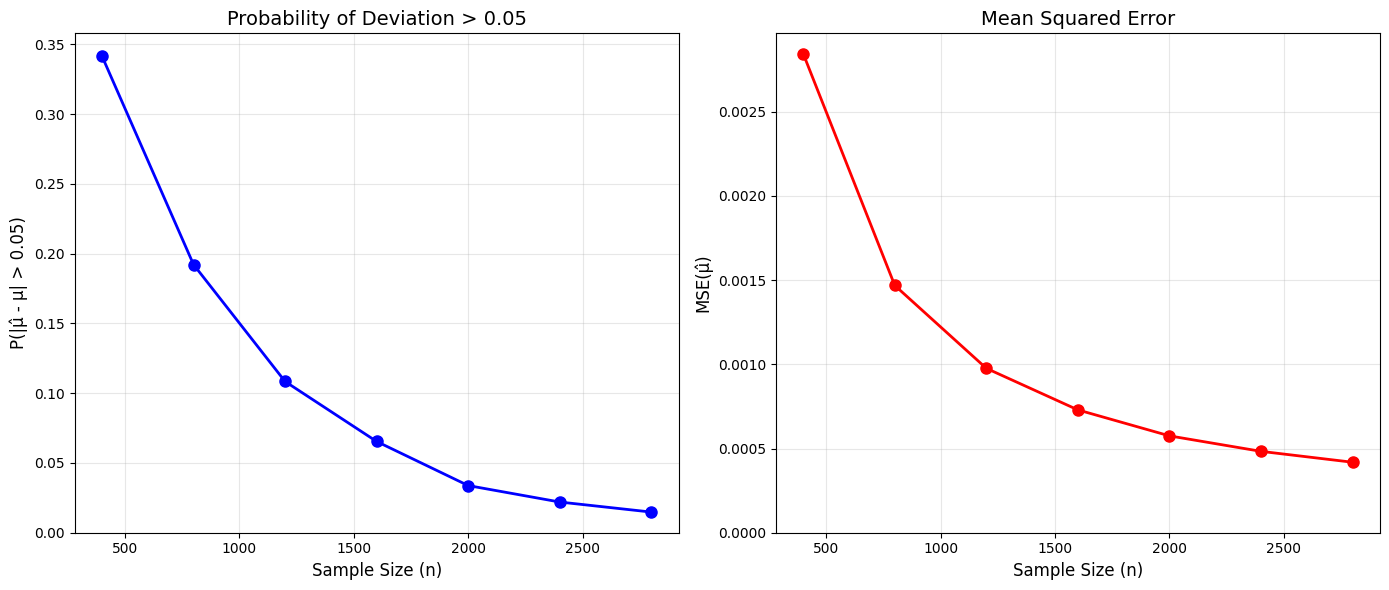
\includegraphics[width=0.8\textwidth]{plot1.png}
    \label{fig:simulation}
\end{figure}
\begin{figure}[h]
    \centering
    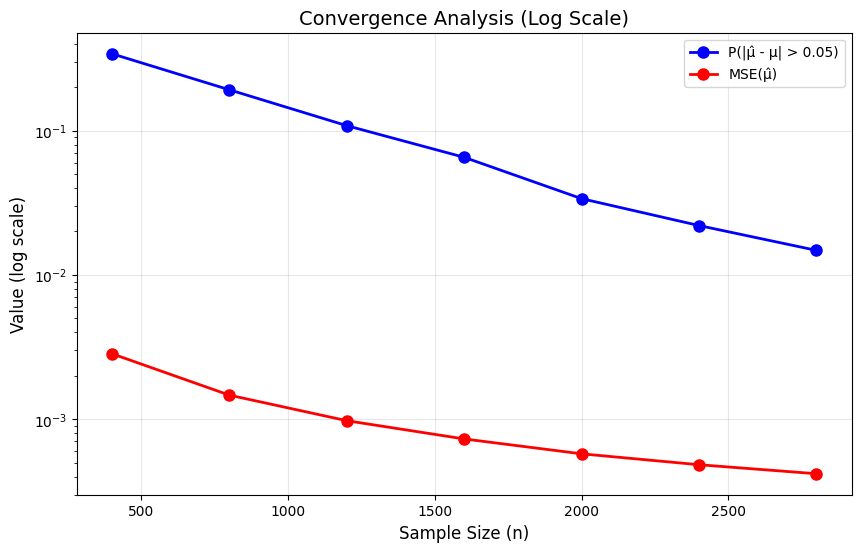
\includegraphics[width=0.5\textwidth]{plot2.png}
    \label{fig:simulation}
\end{figure}
As $n $ increases: 
\begin{itemize}
    \item $P(|\hat{\mu} - \mu| > 0.05) $ decreases to 0 (convergence in probability)
    \item MSE($\hat{\mu}$) decreases to 0 (consistent estimator)
\end{itemize}
This demonstrates the WLLN
\begin{itemize}
    \item The $t(15)$ distribution has finite mean $(\mu = 1)$ and finite variance $(15 / 13 \approxeq 1.154) $
    \item Since $\mathbb{E}[|X_1|] < \infty $, the conditions of the WLLN are satisified
    \item The empirical results confirm that $\hat{\mu}_n \to \mu $ as $n \to \infty $
\end{itemize}
\newpage
20. Prove Corollary 2.6 [Multivariate CLT, i.i.d.]

It states that \textit{If $(X_n)_{n\in \mathbb{N}}$ is an i.i.d. sequence of random vectors with $\text{Var}(X_1) = \Sigma (||\Sigma|| < \infty) $, then for $\mu := \mathbb{E}X_1 $, as $n \to \infty $}
\begin{gather*}
    \frac{1}{\sqrt{n}}\sum_{i = 1}^{n}(X_i - \mu) \xrightarrow{D}\mathcal{N}(0, \Sigma)
\end{gather*}
\textbf{Proof:}

Let $Y_i := X_i - \mu $ and $S_n := \frac{1}{\sqrt{n}}\sum_{i = 1}^{n}Y_i $. Fix $t \in \mathbb{R}^d $. Then the scalar r.vs $t^\top Y_i $ are i.i.d. with mean $0 $ and variance $(t^\top Y_1)=t^\top\Sigma t<\infty$. By the (univariate) central limit theorem,
\begin{gather*}
    t^\top S_n = \frac{1}{\sqrt{n}}\sum_{i = 1}^{n}t^\top Y_i \xrightarrow{D} \mathcal{N}(0, t^\top\Sigma t)
\end{gather*}
Let $Z \sim \mathcal{N}(0, \Sigma)$. Then for every $t \in \mathbb{R}^d, t^\top Z \sim \mathcal{N}(0, t^\top\Sigma t)$. Hence $t^\top S_n \xrightarrow{D}t^\top Z\quad\forall t $. By the Cramér-Wold device (equivalently, Lévy's continuity theorem), this implies $S_n \xrightarrow{D}Z $. Therefore 
\begin{gather*}
    \frac{1}{\sqrt{n}}\sum_{i = 1}^{n}(X_i - \mu) \xrightarrow{D}\mathcal{N}(o, \Sigma)
\end{gather*}
This remains true even if $\Sigma $ is singular (the limit is then a degenerate Gaussian on a subspace). \qed


\end{document}